\documentclass[8pt,apectratio=169]{beamer}

\usetheme[progressbar=frametitle]{metropolis}
\usepackage{appendixnumberbeamer}
\usepackage[style=authoryear, backend=bibtex8, natbib=true, maxcitenames=2]{biblatex}

\usepackage[utf8]{inputenc} % utf8x  defines more symbols, but may cause compatible problems
\usepackage{lmodern,textcomp} % Latin Modern fonts, contains €

\usepackage{graphicx}
\usepackage{import}

\usepackage{booktabs}
\usepackage[scale=2]{ccicons}

\usepackage{pgfplots}
\usepgfplotslibrary{dateplot}

\usepackage{xspace}
\newcommand{\themename}{\textbf{\textsc{metropolis}}\xspace}

% Math
\usepackage{amsmath}
\usepackage{bm} % bold symbol in math mode

% Optional packages
\usepackage{xcolor}
\usepackage{multicol}
\usepackage{hyperref}
\usepackage[super,negative]{nth} % allows writing 1st, 2nd, 3rd with superscript
\usepackage{ulem} % use the "sout" tag to "strikethrough" text
\usepackage{tcolorbox}

% Select what to do with command \comment:
  % \newcommand{\comment}[1]{}  %comments not shown
  % \newcommand{\comment}[1]{\par {\bfseries \color{blue} #1 \par}} %comments shown
% Select what to do with todonotes: i.e. \todo{}, \todo[inline]{}
  % \usepackage[disable]{todonotes} % notes not shown
  % \usepackage[draft]{todonotes}   % notes shown

%\numberwithin{equation}{section}

%\addbibresource{references}

\titlegraphic{\hfill 
\includegraphics[width=0.15 \textwidth]{figures/logo}}
\title{Microeconomics III, Ex. Class 4: Problem Set 1\footnote{Slides created for exercise class 4, with reservation for possible errors.\\}}
\author{Thor Donsby Noe (\href{mailto:thor.noe@econ.ku.dk}{thor.noe@econ.ku.dk})}
\date{September 11 2019} % \today
\institute{\normalsize Department of Economics, University of Copenhagen}

    % \definecolor{BlueTOL}{HTML}{222255}
    \definecolor{BrownTOL}{HTML}{666633}
    \definecolor{GreenTOL}{HTML}{225522}
    % \setbeamercolor{normal text}{fg=BlueTOL,bg=white}
    \setbeamercolor{alerted text}{fg=BrownTOL}
    \setbeamercolor{example text}{fg=GreenTOL}
    \setbeamercolor{background canvas}{bg=white}

    \setbeamercolor{block title alerted}{use=alerted text,
        fg=alerted text.fg,
        bg=alerted text.bg!80!alerted text.fg}
    \setbeamercolor{block body alerted}{use={block title alerted, alerted text},
        fg=alerted text.fg,
        bg=block title alerted.bg!50!alerted text.bg}
    \setbeamercolor{block title example}{use=example text,
        fg=example text.fg,
        bg=example text.bg!80!example text.fg}
    \setbeamercolor{block body example}{use={block title example, example text},
        fg=example text.fg,
        bg=block title example.bg!50!example text.bg}

\begin{document}
\maketitle

% Select what to do with command \intuition{}:
  \newcommand{\intuition}[1]{#1} % intuition shown
  %\newcommand{\intuition}[1]{[...]}  % intuition not shown


% ------------------------------------------------------------------------------
% ------ FRAME -----------------------------------------------------------------
% ------------------------------------------------------------------------------
\begin{frame}{Outline}
    \tableofcontents
\end{frame}


\section{PS12, Ex. 1 (A): Job-market signaling}

\begin{frame}{PS12, Ex. 1 (A): Job-market signaling}
    \begin{multicols}{2}
      \textit{(A)} Consider figure 4.2.8 in Gibbons\\
      (p. 201). Remind yourselves about the separating equilibrium related to the figure. Why can the high type not choose $e^*(H)$ in a separating equilibrium?\vspace{8pt}
      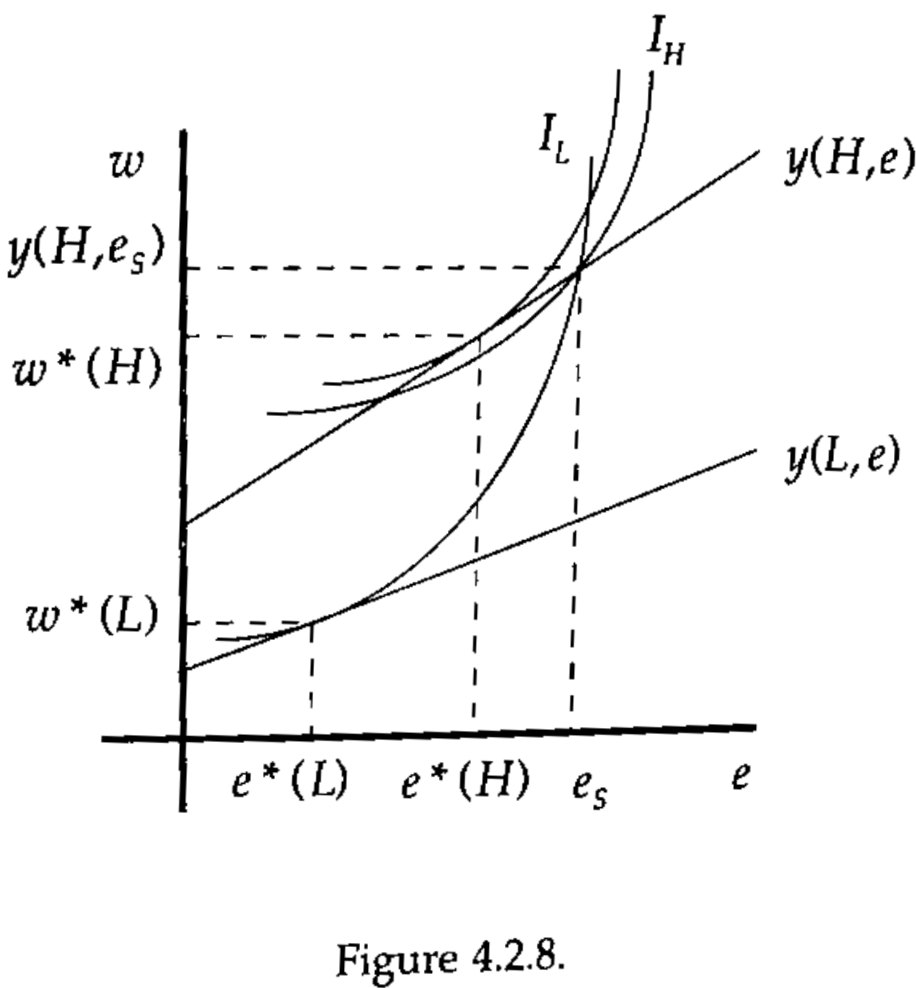
\includegraphics[width=\columnwidth]{figures/Gibbons428}
      \vfill\null\columnbreak
      \begin{itemize}
        \item[Step 1:] \textbf{Explain the graphs $\bm{I_L,I_H,y(L,e),y(H,e)}$.}
      \end{itemize}
      \vfill\null
    \end{multicols}
\end{frame}
\begin{frame}{PS12, Ex. 1 (A): Job-market signaling}
    \begin{multicols}{2}
      \textit{(A)} Consider figure 4.2.8 in Gibbons\\
      (p. 201). Remind yourselves about the separating equilibrium related to the figure. Why can the high type not choose $e^*(H)$ in a separating equilibrium?\vspace{8pt}
      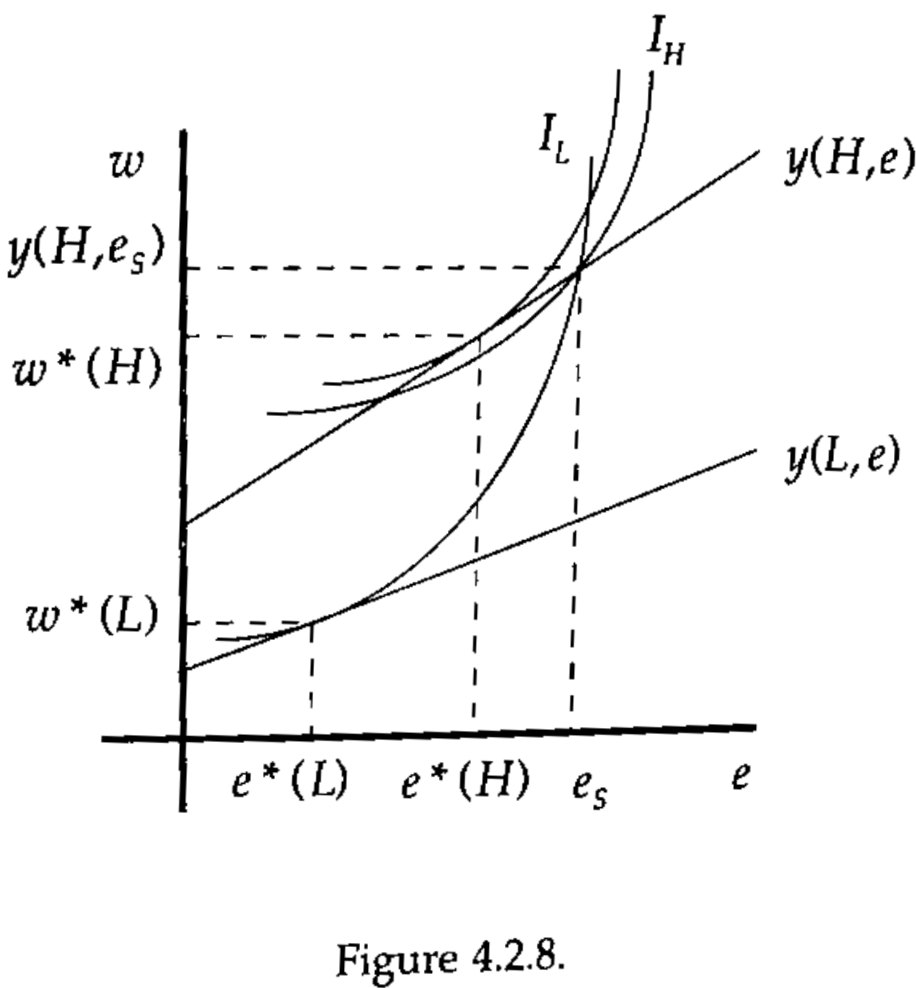
\includegraphics[width=\columnwidth]{figures/Gibbons428}
      \vfill\null\columnbreak
      \begin{itemize}
        \item[Step 1:] Explain $I_L,I_H,y(L,e),y(H,e)$:
      \end{itemize}\vspace{-6pt}
      For each type of worker $\eta\in L,H$:\vspace{-6pt}
      \begin{itemize}
        \item[$I_\eta$:] The indifference curve over which the worker's utility is constant.
        I.e. how much the wage must increase to compensate for higher education.
        \item[$y(\eta,e)$:] \vspace{-2pt} The expected output of a worker with ability $\eta$ and education $e$ which is equal to the wage offered by the firms under competition.\\
        I.e. education is now productive and more so for the high-ability worker.
      \end{itemize}\vspace{-6pt}
      Under complete information, the optimal education is where a worker's indifference curve is tangent to her productivity.\vspace{-6pt}
      \begin{itemize}
        \item[Step 2:] \textbf{Why can \textit{H} not choose $\bm{e^*(H)}$ in a separating equilibrium?}
      \end{itemize}
      \vfill\null
    \end{multicols}
\end{frame}
\begin{frame}{PS12, Ex. 1 (A): Job-market signaling}
    \begin{multicols}{2}
      \textit{(A)} Consider figure 4.2.8 in Gibbons\\
      (p. 201). Remind yourselves about the separating equilibrium related to the figure. Why can the high type not choose $e^*(H)$ in a separating equilibrium?\vspace{8pt}
      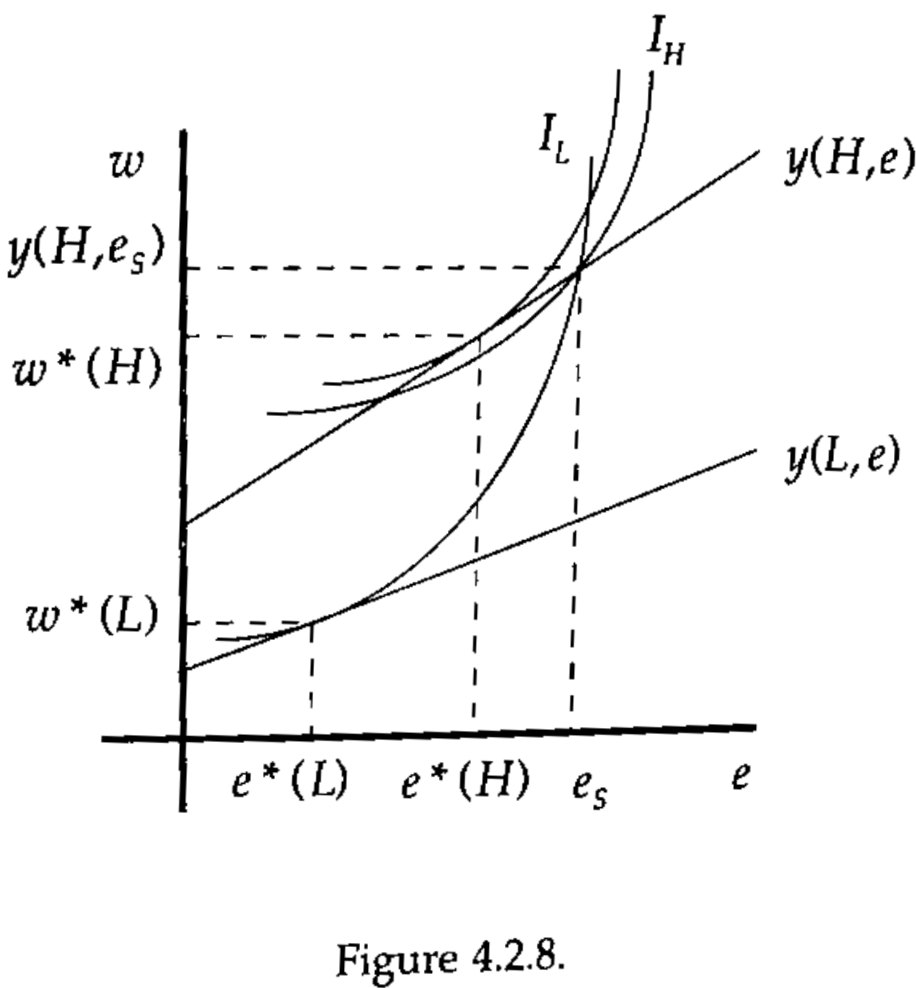
\includegraphics[width=\columnwidth]{figures/Gibbons428}
      \vfill\null\columnbreak
      \begin{itemize}
        \item[Step 1:] Explain $I_L,I_H,y(L,e),y(H,e)$:
      \end{itemize}\vspace{-8pt}
      For each type of worker $\eta\in L,H$:\vspace{-8pt}
      \begin{itemize}
        \item[$I_\eta$:] The indifference curve over which the worker's utility is constant.
        I.e. how much the wage must increase to compensate for higher education.
        \item[$y(\eta,e)$:] \vspace{-4pt} The expected output of a worker with ability $\eta$ and education $e$ which is equal to the wage offered by the firms under competition.\\
        I.e. education is now productive and more so for the high-ability worker.
      \end{itemize}\vspace{-8pt}
      Under complete information, the optimal education is where a worker's indifference curve is tangent to her productivity.\vspace{-8pt}
      \begin{itemize}
        \item[Step 2:] Why can $H$ not choose $e^*(H)$?
      \end{itemize}\vspace{-6pt}
      In a separating equilibrium, the firms perfectly identify $H$ and $L$ by education choices. However, as $[e^*(H),w^*(H)]$ is above $L$'s indifference curve, $L$ would imitate $H$. Thus, $H$ needs to increase education to $e_s$ to credibly signal type $H$.% though this lowers her utility.
      \vfill\null
    \end{multicols}
\end{frame}



\section{PS12, Ex. 2 (A): Farrell \& Rabin (1996): "Cheap talk"}

\begin{frame}{PS12, Ex. 2 (A): Farrell \& Rabin (1996): "Cheap talk"}
    \textit{(A)} In their paper “Cheap Talk” published in the \href{https://www.aeaweb.org/articles?id=10.1257/jep.10.3.103}{\textit{Journal of Economic Perspectives} (1996)}, Joseph Farrell and Matthew Rabin describe the following situation: “Sally knows which one of two tasks is efficient to perform. Rayco [the firm] could hire Sally specifically to perform Job 1, specifically to perform Job 2, or as a highly paid manager who will choose which job to perform. If Rayco knew which task is efficient, it would still hire her to perform the task, but at a lower salary, because she has lost her informational advantage. Sally wants to be hired as manager, but prefers to be hired to do the right task and be more productive rather than to do the wrong task and be less productive.” Payoffs in this situation are\vspace{-6pt}
    \begin{table}
      \begin{tabular}{ll|c|c|c|}
          & \multicolumn{1}{c}{} & \multicolumn{1}{c}{Job 1} & \multicolumn{1}{c}{Job 2} & \multicolumn{1}{c}{Manager} \\\cline{3-5}
          \parbox[t]{20mm}{\multirow{2}{*}{Sally's knowledge}}
           & Task 1 efficient & 2, 5 & 1, -2 & 3, 3 \\\cline{3-5}
           & Task 2 efficient & 1, -2 & 2, 5 & 3, 3 \\\cline{3-5}
      \end{tabular}
    \end{table}\vspace{-2pt}
    where the left number in each cell is Sally’s payoff and the right number is the firm’s payoff (note that this matrix does not describe the normal form of the game!)\vspace{-4pt}
    \begin{itemize}
      \item[(a)] Formulate this strategic situation as a cheap talk game, assuming that the type space is equal to the message space $(T = M)$.
      \item[(b)] Show that a separating equilibrium exists where Sally truthfully reveals which job is efficient, and the firm then places Sally in that specific job.
      \item[(c)] Discuss whether or not this separating equilibrium seems reasonable. Why isn’t Sally able to convince the firm to give her the manager position?
    \end{itemize}\vspace{-6pt}
    \vfill\null
\end{frame}



\subsection{PS12, Ex. 2.a (A): Formulate a cheap talk game}

\begin{frame}{PS12, Ex. 2.a (A): Farrell \& Rabin (1996). Formulate a cheap talk game}
    \begin{table}
      \begin{tabular}{l|c|c|c|}
          \multicolumn{1}{c}{} & \multicolumn{1}{c}{Job 1 $(a=T_1)$} & \multicolumn{1}{c}{Job 2 $(a=T_2)$} & \multicolumn{1}{c}{Manager $(a=Manager)$} \\\cline{2-4}
           Task 1 efficient $(t=T_1)$ & 2, 5 & 1, -2 & 3, 3 \\\cline{2-4}
           Task 2 efficient $(t=T_2)$ & 1, -2 & 2, 5 & 3, 3 \\\cline{2-4}
      \end{tabular}
    \end{table}\vspace{-12pt}
    \begin{itemize}
      \item[(a)] Formulate this strategic situation as a cheap talk game, assuming that the type space is equal to the message space $(T = M)$.
    \end{itemize}\vspace{-6pt}
    \vfill\null
\end{frame}

\begin{frame}{PS12, Ex. 2.a (A): Farrell \& Rabin (1996). Formulate a cheap talk game}
  \begin{table}
    \begin{tabular}{l|c|c|c|}
        \multicolumn{1}{c}{} & \multicolumn{1}{c}{Job 1 $(a=T_1)$} & \multicolumn{1}{c}{Job 2 $(a=T_2)$} & \multicolumn{1}{c}{Manager $(a=Manager)$} \\\cline{2-4}
         Task 1 efficient $(t=T_1)$ & 2, 5 & 1, -2 & 3, 3 \\\cline{2-4}
         Task 2 efficient $(t=T_2)$ & 1, -2 & 2, 5 & 3, 3 \\\cline{2-4}
    \end{tabular}
  \end{table}\vspace{-12pt}
  \begin{itemize}
      \item[(a)] Formulate this strategic situation as a cheap talk game, assuming that the type space is equal to the message space $(T = M)$.
    \end{itemize}\vspace{-6pt}
    The game is as follows:\vspace{-6pt}
    \begin{enumerate}
      \item Sally's type is realized: $t\in\{T_1,T_2\}$, where $t=T_1,T_2$ corresponds to efficiency with Task 1 and Task 2 respectively.
      \item Sally observes her type and sends a cheap talk message $m(t)\in\{T_1,T_2\}$.
      \item Rayco observes the message and chooses a job for Sally: $a(m)\in\{T_1,T_2,M\}$ where $a=T_1,T_2,M$ corresponds to giving Sally one of three jobs:
      \begin{itemize}\normalsize
        \item Job 1 (compatible with task 1 efficiency)
        \item Job 2 (compatible with task 2 efficiency)
        \item Manager (compatible with both but more expensive).
      \end{itemize}
    \end{enumerate}
    \vfill\null
\end{frame}



\subsection{PS12, Ex. 2.b (A): Find a separating PBE}

\begin{frame}{PS12, Ex. 2.b (A): Farrell \& Rabin (1996). Find a separating PBE}
    \begin{table}
      \begin{tabular}{l|c|c|c|}
          \multicolumn{1}{c}{} & \multicolumn{1}{c}{Job 1 $(a=T_1)$} & \multicolumn{1}{c}{Job 2 $(a=T_2)$} & \multicolumn{1}{c}{Manager $(a=Manager)$} \\\cline{2-4}
           Task 1 efficient $(t=T_1)$ & 2, 5 & 1, -2 & 3, 3 \\\cline{2-4}
           Task 2 efficient $(t=T_2)$ & 1, -2 & 2, 5 & 3, 3 \\\cline{2-4}
      \end{tabular}
    \end{table}\vspace{-12pt}
    \begin{itemize}
      \item[(b)] Show that a separating equilibrium exists where Sally truthfully reveals which job is efficient, and the firm then places Sally in that specific job.
    \end{itemize}\vspace{-6pt}
    \vfill\null
\end{frame}
\begin{frame}{PS12, Ex. 2.b (A): Farrell \& Rabin (1996). Find a separating PBE}
    \begin{table}
      \begin{tabular}{l|c|c|c|}
          \multicolumn{1}{c}{} & \multicolumn{1}{c}{Job 1 $(a=T_1)$} & \multicolumn{1}{c}{Job 2 $(a=T_2)$} & \multicolumn{1}{c}{Manager $(a=Manager)$} \\\cline{2-4}
           Task 1 efficient $(t=T_1)$ & 2, 5 & 1, -2 & 3, 3 \\\cline{2-4}
           Task 2 efficient $(t=T_2)$ & 1, -2 & 2, 5 & 3, 3 \\\cline{2-4}
      \end{tabular}
    \end{table}\vspace{-12pt}
    \begin{itemize}
      \item[(b)] Show that a separating equilibrium exists where Sally truthfully reveals which job is efficient, and the firm then places Sally in that specific job.
      \item[Step 1:] \textbf{Go over the beliefs and actions in such a separating PBE. Does either type want to deviate?}
    \end{itemize}
    \vfill\null
\end{frame}
\begin{frame}{PS12, Ex. 2.b (A): Farrell \& Rabin (1996). Find a separating PBE}
    \begin{table}
      \begin{tabular}{l|c|c|c|}
          \multicolumn{1}{c}{} & \multicolumn{1}{c}{Job 1 $(a=T_1)$} & \multicolumn{1}{c}{Job 2 $(a=T_2)$} & \multicolumn{1}{c}{Manager $(a=Manager)$} \\\cline{2-4}
           Task 1 efficient $(t=T_1)$ & 2, 5 & 1, -2 & 3, 3 \\\cline{2-4}
           Task 2 efficient $(t=T_2)$ & 1, -2 & 2, 5 & 3, 3 \\\cline{2-4}
      \end{tabular}
    \end{table}\vspace{-12pt}
    \begin{itemize}
      \item[(b)] Show that a separating equilibrium exists where Sally truthfully reveals which job is efficient, and the firm then places Sally in that specific job.
      \item[Step 1:] Go over the beliefs and actions in such a separating PBE. Does either type want to deviate?
    \end{itemize}\vspace{-6pt}
    In a PBE, the beliefs must correspond to the action of the senders.\\
    Thus in a separating PBE where $m(t=T_1)=T_1$ and $m(t=T_2)=T_2$, beliefs are\vspace{-2pt}
    \begin{align*}
      \mu(t=T_1|m=T_1)=1\text{ and }\mu(t=T_2|m=T_2)=1
    \end{align*}
    This gives R's best responses.
    \vspace{-2pt}
    \begin{align*}
      a(m=T_1)=T_1\text{ and }a(m=T_2)=T_2
    \end{align*}
    Since no message yields the position \textit{Manager}, neither type can imitate the other to get this position, thus, no type has an incentive to deviate.\vspace{-6pt}
    \begin{itemize}
      \item[Step 2:] \textbf{Write up the separating PBE.}
    \end{itemize}
    \vfill\null
\end{frame}
\begin{frame}{PS12, Ex. 2.b (A): Farrell \& Rabin (1996). Find a separating PBE}
    \begin{table}
      \begin{tabular}{l|c|c|c|}
          \multicolumn{1}{c}{} & \multicolumn{1}{c}{Job 1 $(a=T_1)$} & \multicolumn{1}{c}{Job 2 $(a=T_2)$} & \multicolumn{1}{c}{Manager $(a=Manager)$} \\\cline{2-4}
           Task 1 efficient $(t=T_1)$ & 2, 5 & 1, -2 & 3, 3 \\\cline{2-4}
           Task 2 efficient $(t=T_2)$ & 1, -2 & 2, 5 & 3, 3 \\\cline{2-4}
      \end{tabular}
    \end{table}\vspace{-6pt}
    \begin{itemize}
      \item[(b)] Show that a separating equilibrium exists where Sally truthfully reveals which job is efficient, and the firm then places Sally in that specific job.
      \item[Step 1:] Go over the beliefs and actions in such a separating PBE. Does either type want to deviate?
    \end{itemize}\vspace{-6pt}
    In a PBE, the beliefs must correspond to the action of the senders.\\
    Thus in a separating PBE where $m(t=T_1)=T_1$ and $m(t=T_2)=T_2$, beliefs are\vspace{-2pt}
    \begin{align*}
      \mu(t=T_1|m=T_1)=1\text{ and }\mu(t=T_2|m=T_2)=1
    \end{align*}
    This gives R's best responses.
    \vspace{-2pt}
    \begin{align*}
      a(m=T_1)=T_1\text{ and }a(m=T_2)=T_2
    \end{align*}
    Since no message yields the position \textit{Manager}, neither type can imitate the other to get this position, thus, no type has an incentive to deviate.\vspace{-6pt}
    \begin{itemize}
      \item[Step 2:] Write up the separating PBE:
    \end{itemize}\vspace{-6pt}
    \begin{align*}
      \{\underbrace{(T_1,T_2)}_{m(t=T_1),m(t=T_2)},\underbrace{(T_1,T_2)}_{a(m=T_1),a(m=T_2)},\underbrace{\mu(T_1|T_1)=1}_{\mu(t=T_1|m=T_1)},\underbrace{\mu(T_2|T_2)=1}_{\mu(t=T_2|m=T_2)}\}
    \end{align*}
    \vfill\null
\end{frame}


\subsection{PS12, Ex. 2.c (A): Discuss if PBE is reasonable?}

\begin{frame}{PS12, Ex. 2.c (A): Farrell \& Rabin (1996). Discuss if PBE is reasonable?}
    \begin{table}
      \begin{tabular}{l|c|c|c|}
          \multicolumn{1}{c}{} & \multicolumn{1}{c}{Job 1 $(a=T_1)$} & \multicolumn{1}{c}{Job 2 $(a=T_2)$} & \multicolumn{1}{c}{Manager $(a=Manager)$} \\\cline{2-4}
           Task 1 efficient $(t=T_1)$ & 2, 5 & 1, -2 & 3, 3 \\\cline{2-4}
           Task 2 efficient $(t=T_2)$ & 1, -2 & 2, 5 & 3, 3 \\\cline{2-4}
      \end{tabular}
    \end{table}\vspace{-12pt}
    \begin{itemize}
      \item[(c)] Discuss whether or not this separating equilibrium seems reasonable. Why isn’t Sally able to convince the firm to give her the manager position?
    \end{itemize}\vspace{-6pt}
    \begin{multicols}{2}
      \vfill\null\columnbreak
      \vfill\null
    \end{multicols}
\end{frame}
\begin{frame}{PS12, Ex. 2.c (A): Farrell \& Rabin (1996). Discuss if PBE is reasonable?}
    \begin{table}
      \begin{tabular}{l|c|c|c|}
          \multicolumn{1}{c}{} & \multicolumn{1}{c}{Job 1 $(a=T_1)$} & \multicolumn{1}{c}{Job 2 $(a=T_2)$} & \multicolumn{1}{c}{Manager $(a=Manager)$} \\\cline{2-4}
           Task 1 efficient $(t=T_1)$ & 2, 5 & 1, -2 & 3, 3 \\\cline{2-4}
           Task 2 efficient $(t=T_2)$ & 1, -2 & 2, 5 & 3, 3 \\\cline{2-4}
      \end{tabular}
    \end{table}\vspace{-12pt}
    \begin{itemize}
      \item[(c)] Discuss whether or not this separating equilibrium seems reasonable. Why isn’t Sally able to convince the firm to give her the manager position?
      \item[Step 1:] \textbf{Why does Sally not have an incentive to deviate?}
    \end{itemize}
    \vfill\null
\end{frame}
\begin{frame}{PS12, Ex. 2.c (A): Farrell \& Rabin (1996). Discuss if PBE is reasonable?}
    \begin{table}
      \begin{tabular}{l|c|c|c|}
          \multicolumn{1}{c}{} & \multicolumn{1}{c}{Job 1 $(a=T_1)$} & \multicolumn{1}{c}{Job 2 $(a=T_2)$} & \multicolumn{1}{c}{Manager $(a=Manager)$} \\\cline{2-4}
           Task 1 efficient $(t=T_1)$ & 2, 5 & 1, -2 & 3, 3 \\\cline{2-4}
           Task 2 efficient $(t=T_2)$ & 1, -2 & 2, 5 & 3, 3 \\\cline{2-4}
      \end{tabular}
    \end{table}\vspace{-12pt}
    \begin{itemize}
      \item[(c)] Discuss whether or not this separating equilibrium seems reasonable. Why isn’t Sally able to convince the firm to give her the manager position?
      \item[Step 1:] Why does Sally not have an incentive to deviate?
    \end{itemize}\vspace{-6pt}
    Sally has to say that she is efficient at one of the jobs. Since Rayco believe she is telling the truth, she has no choice but to tell the truth, as she would otherwise end up in a worse job for her.
    \vfill\null
\end{frame}
\begin{frame}{PS12, Ex. 2.c (A): Farrell \& Rabin (1996). Discuss if PBE is reasonable?}
    \begin{table}
      \begin{tabular}{l|c|c|c|}
          \multicolumn{1}{c}{} & \multicolumn{1}{c}{Job 1 $(a=T_1)$} & \multicolumn{1}{c}{Job 2 $(a=T_2)$} & \multicolumn{1}{c}{Manager $(a=Manager)$} \\\cline{2-4}
           Task 1 efficient $(t=T_1)$ & 2, 5 & 1, -2 & 3, 3 \\\cline{2-4}
           Task 2 efficient $(t=T_2)$ & 1, -2 & 2, 5 & 3, 3 \\\cline{2-4}
      \end{tabular}
    \end{table}\vspace{-12pt}
    \begin{itemize}
      \item[(c)] Discuss whether or not this separating equilibrium seems reasonable. Why isn’t Sally able to convince the firm to give her the manager position?
      \item[Step 1:] Why does Sally not have an incentive to deviate?
    \end{itemize}\vspace{-6pt}
    Sally has to say that she is efficient at one of the jobs. Since Rayco believe she is telling the truth, she has no choice but to tell the truth, as she would otherwise end up in a worse job for her.\vspace{-6pt}
    \begin{itemize}
      \item[Step 2:] \textbf{Under which circumstances would a pooling PBE exist where both types would get hired as \textit{Manager}?}
    \end{itemize}
    \vfill\null
\end{frame}
\begin{frame}{PS12, Ex. 2.c (A): Farrell \& Rabin (1996). Discuss if PBE is reasonable?}
    \begin{table}
      \begin{tabular}{l|c|c|c|}
          \multicolumn{1}{c}{} & \multicolumn{1}{c}{Job 1 $(a=T_1)$} & \multicolumn{1}{c}{Job 2 $(a=T_2)$} & \multicolumn{1}{c}{Manager $(a=Manager)$} \\\cline{2-4}
           Task 1 efficient $(t=T_1)$ & 2, 5 & 1, -2 & 3, 3 \\\cline{2-4}
           Task 2 efficient $(t=T_2)$ & 1, -2 & 2, 5 & 3, 3 \\\cline{2-4}
      \end{tabular}
    \end{table}\vspace{-6pt}
    \begin{itemize}
      \item[(c)] Discuss whether or not this separating equilibrium seems reasonable. Why isn’t Sally able to convince the firm to give her the manager position?
      \item[Step 1:] Why does Sally not have an incentive to deviate?
    \end{itemize}\vspace{-6pt}
    Sally has to say that she is efficient at one of the jobs. Since Rayco believe she is telling the truth, she has no choice but to tell the truth, as she would otherwise end up in a worse job for her.\vspace{-6pt}
    \begin{itemize}
      \item[Step 2:] Under which circumstances would a pooling PBE exist where both types would get hired as \textit{Manager}?
    \end{itemize}\vspace{-6pt}
    There is a pooling equilibrium where all types of Sally choose the same message ($m=T_1$ or $m=T_2$), thus, don't send any informative signal on what type they are.\\
    In this case, if nature distributes types somewhat equally, i.e. $\mathbb{P}(t=T_1)=p\in\left[\frac{2}{7};\frac{5}{7}\right]$, then the best response for Rayco would be $a(m=T_1)=a(m=T_2)=Manager$ and no type of Sally would want to deviate.
    If nature is very likely to draw type $T_1$ $\left(p>\frac{5}{7}\right)$ then Rayco always offers $T_1$ as $\mathbb{E}[u_\text{R}(a=T_1)]>3$ no matter the signals.
    Likewise, if nature is unlikely to draw $T_1$ $\left(p<\frac{2}{7}\right)$ then $\mathbb{E}[u_\text{R}(a=T_2)]>3$.\\
    I.e. the separating PBE would be realistic if each type made a strategy in isolation. However, as Sally constitutes all types, she can decide on a tactic for all type of senders. No type would want to deviate from the pooling PBE $\left(\text{for }p\in\left[\frac{2}{7};\frac{5}{7}\right]\right)$.
    \vfill\null
\end{frame}



\section{PS12, Ex. 3: Cheap talk games (extensive form)}

\begin{frame}{PS12, Ex. 3: Cheap talk games (extensive form)}
    Consider the games (a)-(d) on the next page. (i) Which of these are cheap talk games? (ii) For those which are cheap talk games, find a separating equilibrium if such an equilibrium exists, or show that no separating equilibrium exists.
    \vfill\null
\end{frame}

\begin{frame}{PS12, Ex. 3.i: Cheap talk games (extensive form)}
    (ii) Which of these are cheap talk games?\vspace{-6pt}
    \begin{multicols}{2}
      \begin{figure}[!h]
        \center\def\svgwidth{1\columnwidth}
        \import{figures/}{3a.pdf_tex}
      \end{figure}\vspace{-6pt}
      \begin{figure}[!h]
        \center\def\svgwidth{1\columnwidth}
        \import{figures/}{3b.pdf_tex}
      \end{figure}
      \vfill\null\columnbreak
      \begin{figure}[!h]
        \center\def\svgwidth{1\columnwidth}
        \import{figures/}{3c.pdf_tex}
      \end{figure}\vspace{-6pt}
      \begin{figure}[!h]
        \center\def\svgwidth{1\columnwidth}
        \import{figures/}{3d.pdf_tex}
      \end{figure}
      \vfill\null
    \end{multicols}
\end{frame}
\begin{frame}{PS12, Ex. 3.i: Cheap talk games (extensive form)}
    (ii) In cheap talk games, payoffs don't depend on the message: $u_\text{S}(t_i,a_k),u_\text{R}(t_i,a_k)$.\vspace{-6pt}
    \begin{multicols}{2}
      \begin{figure}[!h]
        \center\def\svgwidth{1\columnwidth}
        \import{figures/}{3a.pdf_tex}
      \end{figure}\vspace{-6pt}
      \begin{figure}[!h]
        \center\def\svgwidth{1\columnwidth}
        \import{figures/}{3b.pdf_tex}
      \end{figure}
      \vfill\null\columnbreak
      \begin{figure}[!h]
        \center\def\svgwidth{1\columnwidth}
        \import{figures/}{3c.pdf_tex}
      \end{figure}\vspace{-6pt}
      \begin{figure}[!h]
        \center\def\svgwidth{1\columnwidth}
        \import{figures/}{3d.pdf_tex}
      \end{figure}
      \vfill\null
    \end{multicols}
\end{frame}
\begin{frame}{PS12, Ex. 3.i: Cheap talk games (extensive form)}
    (ii) In (a) and (d) signals are "cheap" as all payoffs are the same for $L$ and $R$:\vspace{-14pt}
    \begin{multicols}{2}
      \vfill\null\vspace{-10.2pt}
      \begin{figure}[!h]
        \center\def\svgwidth{1\columnwidth}
        \import{figures/}{3a.pdf_tex}
      \end{figure}\vspace{-20.3pt}
      \begin{figure}[!h]
        \center\def\svgwidth{1.41\columnwidth}
        \import{figures/}{3b_red.pdf_tex}
      \end{figure}
      \vfill\null\columnbreak
      \begin{figure}[!h]
        \center\def\svgwidth{1.26\columnwidth}
        \import{figures/}{3c_red.pdf_tex}
      \end{figure}\vspace{-9pt}
      \begin{figure}[!h]
        \center\def\svgwidth{1\columnwidth}
        \import{figures/}{3d.pdf_tex}
      \end{figure}
      \vfill\null
    \end{multicols}
\end{frame}

\begin{frame}{PS12, Ex. 3.ii: Cheap talk games (extensive form)}
    (ii) For those which are cheap talk games [(a) and (d)], find a separating equilibrium if such an equilibrium exists, or show that no separating equilibrium exists.\vspace{-6pt}
    \begin{multicols}{2}
      \begin{figure}[!h]
        \center\def\svgwidth{1\columnwidth}
        \import{figures/}{3a.pdf_tex}
      \end{figure}
      \vfill\null\columnbreak
      \vfill\null\vspace{85pt}
      \begin{figure}[!h]
        \center\def\svgwidth{1\columnwidth}
        \import{figures/}{3d.pdf_tex}
      \end{figure}
    \end{multicols}
\end{frame}

\begin{frame}{PS12, Ex. 3.ii.a: Cheap talk games (extensive form)}
    (ii) For those which are cheap talk games, find a separating equilibrium if such an equilibrium exists, or show that no separating equilibrium exists.\vspace{-6pt}
    \begin{multicols}{2}
      \begin{figure}[!h]
        \center\def\svgwidth{1.1\columnwidth}
        \import{figures/}{3a.pdf_tex}
      \end{figure}\vspace{-6pt}
      \begin{itemize}
        \item[Step 1:] \textbf{For the separating strategy (\textit{L,R}), go over SR3, SR2R, and SR2S. PBE?}
        \item[Step 2:] For the separating strategy (\textit{R,L}), go over SR3, SR2R, and SR2S. PBE?
      \end{itemize}
      \vfill\null\columnbreak
      \vfill\null
    \end{multicols}
\end{frame}
\begin{frame}{PS12, Ex. 3.ii.a: Cheap talk games (extensive form)}
    (ii) For those which are cheap talk games, find a separating equilibrium if such an equilibrium exists, or show that no separating equilibrium exists.\vspace{-6pt}
    \begin{multicols}{2}
      \begin{figure}[!h]
        \center\def\svgwidth{1.1\columnwidth}
        \import{figures/}{3a_LR_ud.pdf_tex}
      \end{figure}\vspace{-6pt}
      \begin{itemize}
        \item[Step 1:] For the separating strategy (\textit{L,R}), go over SR3, SR2R, and SR2S. PBE?
        \item[Step 2:] \textbf{For the separating strategy (\textit{R,L}), go over SR3, SR2R, and SR2S. PBE?}
      \end{itemize}
      \vfill\null\columnbreak
      \begin{enumerate}
        \item SR3: R: Beliefs given S's strategy:\vspace{-8pt}
        \begin{align*}
          \mu(t_1|L)=p=1\text{ and }\mu(t_1|R)=q=0
        \end{align*}\vspace{-18pt}
        \begin{itemize}\normalsize
          \item[SR2R:] R: $a^*(L)=u,\ a^*(R)=d$.
          \item[SR2S:] $t_1$ will not deviate if
        \end{itemize}\vspace{-10pt}
        \begin{align*}
          u_\text{S}(L,u|t_1)=3\geq a=u_\text{S}(R,d|t_1)
        \end{align*}\vspace{-18pt}
        \begin{itemize}\normalsize
          \item[] $t_2$ will never deviate as
        \end{itemize}\vspace{-10pt}
        \begin{align*}
          u_\text{S}(R,d|t_2)=5>2=u_\text{S}(L,u|t_2)
        \end{align*}\vspace{-18pt}
        \begin{itemize}\normalsize
          \item[PBE:] No deviation if $a\leq3$ \textcolor{Pink}{(pink)}.
        \end{itemize}
      \end{enumerate}
      \vfill\null
    \end{multicols}
\end{frame}
\begin{frame}{PS12, Ex. 3.ii.a: Cheap talk games (extensive form)}
    (ii) For those which are cheap talk games, find a separating equilibrium if such an equilibrium exists, or show that no separating equilibrium exists.\vspace{-6pt}
    \begin{multicols}{2}
      \begin{figure}[!h]
        \center\def\svgwidth{1.1\columnwidth}
        \import{figures/}{3a_RL_du.pdf_tex}
      \end{figure}\vspace{-6pt}
      \begin{itemize}
        \item[Step 1:] For the separating strategy (\textit{L,R}), go over SR3, SR2R, and SR2S. PBE?
        \item[Step 2:] For the separating strategy (\textit{R,L}), go over SR3, SR2R, and SR2S. PBE?
        \item[Step 3:] \textbf{Write up the set of separating PBE.}
      \end{itemize}
      \vfill\null\columnbreak
      \begin{enumerate}
        \item SR3: R: Beliefs given S's strategy:\vspace{-8pt}
        \begin{align*}
          \mu(t_1|L)=p=1\text{ and }\mu(t_1|R)=q=0
        \end{align*}\vspace{-18pt}
        \begin{itemize}\normalsize
          \item[SR2R:] R: $a^*(L)=u,\ a^*(R)=d$.
          \item[SR2S:] $t_1$ will not deviate if
        \end{itemize}\vspace{-10pt}
        \begin{align*}
          u_\text{S}(L,u|t_1)=3\geq a=u_\text{S}(R,d|t_1)
        \end{align*}\vspace{-18pt}
        \begin{itemize}\normalsize
          \item[] $t_2$ will never deviate as
        \end{itemize}\vspace{-10pt}
        \begin{align*}
          u_\text{S}(R,d|t_2)=5>2=u_\text{S}(L,u|t_2)
        \end{align*}\vspace{-18pt}
        \begin{itemize}\normalsize
          \item[PBE:] No deviation if $a\leq3$ \textcolor{Pink}{(pink)}.
        \end{itemize}
        \item SR3: R: Beliefs given S's strategy:\vspace{-8pt}
        \begin{align*}
          \mu(t_1|L)=p=0\text{ and }\mu(t_1|R)=q=1
        \end{align*}\vspace{-18pt}
        \begin{itemize}\normalsize
          \item[SR2R:] R: $a^*(L)=d,\ a^*(R)=u$.
          \item[SR2S:] $t_1$ will not deviate if
        \end{itemize}\vspace{-10pt}
        \begin{align*}
          u_\text{S}(R,u|t_1)=3\geq a=u_\text{S}(L,d|t_1)
        \end{align*}\vspace{-18pt}
        \begin{itemize}\normalsize
          \item[] $t_2$ will never deviate as
        \end{itemize}\vspace{-10pt}
        \begin{align*}
          u_\text{S}(L,d|t_2)=5>2=u_\text{S}(R,u|t_2)
        \end{align*}\vspace{-18pt}
        \begin{itemize}\normalsize
          \item[PBE:] No deviation if $a\leq3$ \textcolor{green}{(green)}.
        \end{itemize}
      \end{enumerate}
      \vfill\null
    \end{multicols}
\end{frame}
\begin{frame}{PS12, Ex. 3.ii.a: Cheap talk games (extensive form)}
    (ii) For those which are cheap talk games, find a separating equilibrium if such an equilibrium exists, or show that no separating equilibrium exists.\vspace{-10pt}
    \begin{multicols}{2}
      \begin{figure}[!h]
        \center\def\svgwidth{1.1\columnwidth}
        \import{figures/}{3a_LR-RL.pdf_tex}
      \end{figure}\vspace{-6pt}
      \begin{itemize}
        \item[Step 1:] For the separating strategy (\textit{L,R}), go over SR3, SR2R, and SR2S. PBE?
        \item[Step 2:] For the separating strategy (\textit{R,L}), go over SR3, SR2R, and SR2S. PBE?
        \item[Step 3:] Write up the set of separating PBE.
        \item[Step 4:] \textbf{Is S's "cheap talk" informative? How is/isn't that possible?}
      \end{itemize}
      \vfill\null\columnbreak
      \begin{enumerate}
        \item SR3: R: Beliefs given S's strategy:\vspace{-8pt}
        \begin{align*}
          \mu(t_1|L)=p=1\text{ and }\mu(t_1|R)=q=0
        \end{align*}\vspace{-18pt}
        \begin{itemize}\normalsize
          \item[SR2R:] R: $a^*(L)=u,\ a^*(R)=d$.
          \item[SR2S:] $t_1$ will not deviate if
        \end{itemize}\vspace{-10pt}
        \begin{align*}
          u_\text{S}(L,u|t_1)=3\geq a=u_\text{S}(R,d|t_1)
        \end{align*}\vspace{-18pt}
        \begin{itemize}\normalsize
          \item[] $t_2$ will never deviate as
        \end{itemize}\vspace{-10pt}
        \begin{align*}
          u_\text{S}(R,d|t_2)=5>2=u_\text{S}(L,u|t_2)
        \end{align*}\vspace{-18pt}
        \begin{itemize}\normalsize
          \item[PBE:] No deviation if $a\leq3$ \textcolor{Pink}{(pink)}.
        \end{itemize}
        \item SR3: R: Beliefs given S's strategy:\vspace{-8pt}
        \begin{align*}
          \mu(t_1|L)=p=0\text{ and }\mu(t_1|R)=q=1
        \end{align*}\vspace{-18pt}
        \begin{itemize}\normalsize
          \item[SR2R:] R: $a^*(L)=d,\ a^*(R)=u$.
          \item[SR2S:] $t_1$ will not deviate if
        \end{itemize}\vspace{-10pt}
        \begin{align*}
          u_\text{S}(R,u|t_1)=3\geq a=u_\text{S}(L,d|t_1)
        \end{align*}\vspace{-18pt}
        \begin{itemize}\normalsize
          \item[] $t_2$ will never deviate as
        \end{itemize}\vspace{-10pt}
        \begin{align*}
          u_\text{S}(L,d|t_2)=5>2=u_\text{S}(R,u|t_2)
        \end{align*}\vspace{-18pt}
        \begin{itemize}\normalsize
          \item[PBE:] No deviation if $a\leq3$ \textcolor{green}{(green)}.
        \end{itemize}
        \item Two separating PBE exist for $a\leq3$:\vspace{-8pt}
        \begin{align*}
          PBE=\left\{\begin{array}{c}
              (L,R),(u,d),p=1,q=0\\
              (R,L),(d,u),p=0,q=1\end{array}\right\}
        \end{align*}
      \end{enumerate}
      \vfill\null
    \end{multicols}
\end{frame}
\begin{frame}{PS12, Ex. 3.ii.a: Cheap talk games (extensive form)}
    \begin{multicols}{2}
      \begin{figure}[!h]
        \center\def\svgwidth{1.1\columnwidth}
        \import{figures/}{3a_LR-RL.pdf_tex}
      \end{figure}\vspace{-8pt}
      \begin{itemize}
        \item[Step 1:] For the separating strategy (\textit{L,R}), go over SR3, SR2R, and SR2S. PBE?
        \item[Step 2:] \vspace{-2pt}For the separating strategy (\textit{R,L}), go over SR3, SR2R, and SR2S. PBE?
        \item[Step 3:] \vspace{-2pt}Write up the set of separating PBE.
        \item[Step 4:] \vspace{-2pt}S's "cheap talk" is informative as:
      \end{itemize}\vspace{-6pt}
      (1) $t_1$ and $t_2$ prefer different actions, (2) R prefers different actions for different sender types, and (3) S’s types and R’s preferences are aligned.
      \vfill\null\columnbreak
      \begin{enumerate}
        \item SR3: R: Beliefs given S's strategy:\vspace{-8pt}
        \begin{align*}
          \mu(t_1|L)=p=1\text{ and }\mu(t_1|R)=q=0
        \end{align*}\vspace{-18pt}
        \begin{itemize}\normalsize
          \item[SR2R:] R: $a^*(L)=u,\ a^*(R)=d$.
          \item[SR2S:] $t_1$ will not deviate if
        \end{itemize}\vspace{-10pt}
        \begin{align*}
          u_\text{S}(L,u|t_1)=3\geq a=u_\text{S}(R,d|t_1)
        \end{align*}\vspace{-18pt}
        \begin{itemize}\normalsize
          \item[] $t_2$ will never deviate as
        \end{itemize}\vspace{-10pt}
        \begin{align*}
          u_\text{S}(R,d|t_2)=5>2=u_\text{S}(L,u|t_2)
        \end{align*}\vspace{-18pt}
        \begin{itemize}\normalsize
          \item[PBE:] No deviation if $a\leq3$ \textcolor{Pink}{(pink)}.
        \end{itemize}
        \item SR3: R: Beliefs given S's strategy:\vspace{-8pt}
        \begin{align*}
          \mu(t_1|L)=p=0\text{ and }\mu(t_1|R)=q=1
        \end{align*}\vspace{-18pt}
        \begin{itemize}\normalsize
          \item[SR2R:] R: $a^*(L)=d,\ a^*(R)=u$.
          \item[SR2S:] $t_1$ will not deviate if
        \end{itemize}\vspace{-10pt}
        \begin{align*}
          u_\text{S}(R,u|t_1)=3\geq a=u_\text{S}(L,d|t_1)
        \end{align*}\vspace{-18pt}
        \begin{itemize}\normalsize
          \item[] $t_2$ will never deviate as
        \end{itemize}\vspace{-10pt}
        \begin{align*}
          u_\text{S}(L,d|t_2)=5>2=u_\text{S}(R,u|t_2)
        \end{align*}\vspace{-18pt}
        \begin{itemize}\normalsize
          \item[PBE:] No deviation if $a\leq3$ \textcolor{green}{(green)}.
        \end{itemize}
        \item Two separating PBE exist for $a\leq3$:\vspace{-8pt}
        \begin{align*}
          PBE=\left\{\begin{array}{c}
              (L,R),(u,d),p=1,q=0\\
              (R,L),(d,u),p=0,q=1\end{array}\right\}
        \end{align*}
      \end{enumerate}
      \vfill\null
    \end{multicols}
\end{frame}

\begin{frame}{PS12, Ex. 3.ii.d: Cheap talk games (extensive form)}
    (ii) For those which are cheap talk games, find a separating equilibrium if such an equilibrium exists, or show that no separating equilibrium exists.\vspace{-6pt}
    \begin{multicols}{2}
      \begin{figure}[!h]
        \center\def\svgwidth{1.1\columnwidth}
        \import{figures/}{3d.pdf_tex}
      \end{figure}\vspace{-6pt}
      \begin{itemize}
        \item[Step 1:] \textbf{For the separating strategy (\textit{L,R}), go over SR3, SR2R, and SR2S. PBE?}
        \item[Step 2:] For the separating strategy (\textit{R,L}), go over SR3, SR2R, and SR2S. PBE?
      \end{itemize}
      \vfill\null\columnbreak
      \vfill\null
    \end{multicols}
\end{frame}
\begin{frame}{PS12, Ex. 3.ii.d: Cheap talk games (extensive form)}
    (ii) For those which are cheap talk games, find a separating equilibrium if such an equilibrium exists, or show that no separating equilibrium exists.\vspace{-6pt}
    \begin{multicols}{2}
      \begin{figure}[!h]
        \center\def\svgwidth{1.1\columnwidth}
        \import{figures/}{3d_LR_uu.pdf_tex}
      \end{figure}\vspace{-6pt}
      \begin{itemize}
        \item[Step 1:] For the separating strategy (\textit{L,R}), go over SR3, SR2R, and SR2S. PBE?
        \item[Step 2:] \textbf{For the separating strategy (\textit{R,L}), go over SR3, SR2R, and SR2S. PBE?}
      \end{itemize}
      \vfill\null\columnbreak
      \begin{enumerate}
        \item SR3: R: Beliefs given S's strategy:\vspace{-8pt}
        \begin{align*}
          \mu(t_1|L)=p=1\text{ and }\mu(t_1|R)=q=0
        \end{align*}\vspace{-18pt}
        \begin{itemize}\normalsize
          \item[SR2R:] R: $a^*(L)=u,\ a^*(R)=u$.
          \item[SR2S:] $t_1$ will not deviate if
        \end{itemize}\vspace{-10pt}
        \begin{align*}
          u_\text{S}(L,u|t_1)=3\geq 3=u_\text{S}(R,u|t_1)
        \end{align*}\vspace{-18pt}
        \begin{itemize}\normalsize
          \item[] $t_2$ will never deviate as
        \end{itemize}\vspace{-10pt}
        \begin{align*}
          u_\text{S}(R,u|t_2)=3>3=u_\text{S}(L,u|t_2)
        \end{align*}\vspace{-18pt}
        \begin{itemize}\normalsize
          \item[PBE:] No deviation $\rightarrow$ PBE \textcolor{YellowOrange}{(orange)}.
        \end{itemize}
      \end{enumerate}
      \vfill\null
    \end{multicols}
\end{frame}
\begin{frame}{PS12, Ex. 3.ii.d: Cheap talk games (extensive form)}
    (ii) For those which are cheap talk games, find a separating equilibrium if such an equilibrium exists, or show that no separating equilibrium exists.\vspace{-6pt}
    \begin{multicols}{2}
      \begin{figure}[!h]
        \center\def\svgwidth{1.1\columnwidth}
        \import{figures/}{3d_RL_uu.pdf_tex}
      \end{figure}\vspace{-6pt}
      \begin{itemize}
        \item[Step 1:] For the separating strategy (\textit{L,R}), go over SR3, SR2R, and SR2S. PBE?
        \item[Step 2:] For the separating strategy (\textit{R,L}), go over SR3, SR2R, and SR2S. PBE?
        \item[Step 3:] \textbf{Write up the full set of separating PBE.}
      \end{itemize}
      \vfill\null\columnbreak
      \begin{enumerate}
        \item SR3: R: Beliefs given S's strategy:\vspace{-8pt}
        \begin{align*}
          \mu(t_1|L)=p=1\text{ and }\mu(t_1|R)=q=0
        \end{align*}\vspace{-18pt}
        \begin{itemize}\normalsize
          \item[SR2R:] R: $a^*(L)=u,\ a^*(R)=u$.
          \item[SR2S:] $t_1$ will not deviate if
        \end{itemize}\vspace{-10pt}
        \begin{align*}
          u_\text{S}(L,u|t_1)=3\geq 3=u_\text{S}(R,u|t_1)
        \end{align*}\vspace{-18pt}
        \begin{itemize}\normalsize
          \item[] $t_2$ will never deviate as
        \end{itemize}\vspace{-10pt}
        \begin{align*}
          u_\text{S}(R,u|t_2)=3\geq3=u_\text{S}(L,u|t_2)
        \end{align*}\vspace{-18pt}
        \begin{itemize}\normalsize
          \item[PBE:] No deviation $\rightarrow$ PBE \textcolor{YellowOrange}{(orange)}.
        \end{itemize}
        \item SR3: R: Beliefs given S's strategy:\vspace{-8pt}
        \begin{align*}
          \mu(t_1|L)=p=0\text{ and }\mu(t_1|R)=q=1
        \end{align*}\vspace{-18pt}
        \begin{itemize}\normalsize
          \item[SR2R:] R: $a^*(L)=u,\ a^*(R)=u$.
          \item[SR2S:] $t_1$ will not deviate as
        \end{itemize}\vspace{-10pt}
        \begin{align*}
          u_\text{S}(R,u|t_1)=3\geq 3=u_\text{S}(L,u|t_1)
        \end{align*}\vspace{-18pt}
        \begin{itemize}\normalsize
          \item[] $t_2$ will not deviate as
        \end{itemize}\vspace{-10pt}
        \begin{align*}
          u_\text{S}(L,u|t_2)=3\geq3=u_\text{S}(R,u|t_2)
        \end{align*}\vspace{-18pt}
        \begin{itemize}\normalsize
          \item[PBE:] No deviation $\rightarrow$ PBE \textcolor{blue}{(blue)}.
        \end{itemize}
      \end{enumerate}
      \vfill\null
    \end{multicols}
\end{frame}
\begin{frame}{PS12, Ex. 3.ii.d: Cheap talk games (extensive form)}
    (ii) For those which are cheap talk games, find a separating equilibrium if such an equilibrium exists, or show that no separating equilibrium exists.\vspace{-10pt}
    \begin{multicols}{2}
      \begin{figure}[!h]
        \center\def\svgwidth{1.1\columnwidth}
        \import{figures/}{3d_LR-RL_uu.pdf_tex}
      \end{figure}\vspace{-6pt}
      \begin{itemize}
        \item[Step 1:] For the separating strategy (\textit{L,R}), go over SR3, SR2R, and SR2S. PBE?
        \item[Step 2:] \vspace{-1pt}For the separating strategy (\textit{R,L}), go over SR3, SR2R, and SR2S. PBE?
        \item[Step 3:] \vspace{-1pt}Write up the full set of separating PBE.
        \item[Step 4:] \vspace{-1pt}\textbf{Explain. Why are the signals non-informative "cheap talk"?}
      \end{itemize}
      \vfill\null\columnbreak
      \begin{enumerate}
        \item SR3: R: Beliefs given S's strategy:\vspace{-8pt}
        \begin{align*}
          \mu(t_1|L)=p=1\text{ and }\mu(t_1|R)=q=0
        \end{align*}\vspace{-18pt}
        \begin{itemize}\normalsize
          \item[SR2R:] R: $a^*(L)=u,\ a^*(R)=u$.
          \item[SR2S:] $t_1$ will not deviate if
        \end{itemize}\vspace{-10pt}
        \begin{align*}
          u_\text{S}(L,u|t_1)=3\geq 3=u_\text{S}(R,u|t_1)
        \end{align*}\vspace{-18pt}
        \begin{itemize}\normalsize
          \item[] $t_2$ will never deviate as
        \end{itemize}\vspace{-10pt}
        \begin{align*}
          u_\text{S}(R,u|t_2)=3\geq3=u_\text{S}(L,u|t_2)
        \end{align*}\vspace{-18pt}
        \begin{itemize}\normalsize
          \item[PBE:] No deviation $\rightarrow$ PBE \textcolor{YellowOrange}{(orange)}.
        \end{itemize}
        \item SR3: R: Beliefs given S's strategy:\vspace{-8pt}
        \begin{align*}
          \mu(t_1|L)=p=0\text{ and }\mu(t_1|R)=q=1
        \end{align*}\vspace{-18pt}
        \begin{itemize}\normalsize
          \item[SR2R:] R: $a^*(L)=u,\ a^*(R)=u$.
          \item[SR2S:] $t_1$ will not deviate as
        \end{itemize}\vspace{-10pt}
        \begin{align*}
          u_\text{S}(R,u|t_1)=3\geq 3=u_\text{S}(L,u|t_1)
        \end{align*}\vspace{-18pt}
        \begin{itemize}\normalsize
          \item[] $t_2$ will not deviate as
        \end{itemize}\vspace{-10pt}
        \begin{align*}
          u_\text{S}(L,u|t_2)=3\geq3=u_\text{S}(R,u|t_2)
        \end{align*}\vspace{-18pt}
        \begin{itemize}\normalsize
          \item[PBE:] No deviation $\rightarrow$ PBE \textcolor{blue}{(blue)}.
        \end{itemize}
        \item $\left\{\begin{array}{c}
            (L,R),(u,u),p=1,q=0\\
            (R,L),(u,u),p=0,q=1\end{array}\right\}$
      \end{enumerate}
      \vfill\null
    \end{multicols}
\end{frame}
\begin{frame}{PS12, Ex. 3.ii.d: Cheap talk games (extensive form)}
    \begin{multicols}{2}
      \begin{figure}[!h]
        \center\def\svgwidth{1.1\columnwidth}
        \import{figures/}{3d_LR-RL_uu.pdf_tex}
      \end{figure}\vspace{-6pt}
      \begin{itemize}
        \item[Step 1:] For the separating strategy (\textit{L,R}), go over SR3, SR2R, and SR2S. PBE?
        \item[Step 2:] For the separating strategy (\textit{R,L}), go over SR3, SR2R, and SR2S. PBE?
        \item[Step 3:] Write up the full set of separating PBE.
        \item[Step 4:] Explain. Why are the signals non-informative "cheap talk"?
      \end{itemize}
      \vfill\null\columnbreak
      \begin{enumerate}
        \item SR3: R: Beliefs given S's strategy:\vspace{-8pt}
        \begin{align*}
          \mu(t_1|L)=p=1\text{ and }\mu(t_1|R)=q=0
        \end{align*}\vspace{-18pt}
        \begin{itemize}\normalsize
          \item[SR2R:] R: $a^*(L)=u,\ a^*(R)=u$.
          \item[SR2S:] $t_1$ will not deviate if
        \end{itemize}\vspace{-10pt}
        \begin{align*}
          u_\text{S}(L,u|t_1)=3\geq 3=u_\text{S}(R,u|t_1)
        \end{align*}\vspace{-18pt}
        \begin{itemize}\normalsize
          \item[] $t_2$ will never deviate as
        \end{itemize}\vspace{-10pt}
        \begin{align*}
          u_\text{S}(R,u|t_2)=3\geq3=u_\text{S}(L,u|t_2)
        \end{align*}\vspace{-18pt}
        \begin{itemize}\normalsize
          \item[PBE:] No deviation $\rightarrow$ PBE \textcolor{YellowOrange}{(orange)}.
        \end{itemize}\vspace{-5pt}
        \item SR3: R: Beliefs given S's strategy:\vspace{-8pt}
        \begin{align*}
          \mu(t_1|L)=p=0\text{ and }\mu(t_1|R)=q=1
        \end{align*}\vspace{-18pt}
        \begin{itemize}\normalsize
          \item[SR2R:] R: $a^*(L)=u,\ a^*(R)=u$.
          \item[SR2S:] $t_1$ will not deviate as
        \end{itemize}\vspace{-10pt}
        \begin{align*}
          u_\text{S}(R,u|t_1)=3\geq 3=u_\text{S}(L,u|t_1)
        \end{align*}\vspace{-18pt}
        \begin{itemize}\normalsize
          \item[] $t_2$ will not deviate as
        \end{itemize}\vspace{-10pt}
        \begin{align*}
          u_\text{S}(L,u|t_2)=3\geq3=u_\text{S}(R,u|t_2)
        \end{align*}\vspace{-18pt}
        \begin{itemize}\normalsize
          \item[PBE:] No deviation $\rightarrow$ PBE \textcolor{blue}{(blue)}.
        \end{itemize}\vspace{-4pt}
        \item $\left\{\begin{array}{c}
            (L,R),(u,u),p=1,q=0\\
            (R,L),(u,u),p=0,q=1\end{array}\right\}$
        \item \vspace{-1pt}Two "weak separating PBE": Both $t_1$ and $t_2$ is indifferent between signals as R will always choose $u$.
      \end{enumerate}
      \vfill\null
    \end{multicols}
\end{frame}



\section{PS12, Ex. 4: Three-type job-applicant cheap talk game}

\begin{frame}{PS12, Ex. 4: Three-type job-applicant cheap talk game}
    Consider the following job-applicant cheap talk game based on \href{https://www.aeaweb.org/articles?id=10.1257/jep.10.3.103}{Farrell-Rabin (1996)}. Suppose that there are three types of potential applicants (high ability, medium ability, and low ability) and the firm can place the applicant in one of threeH possible positions (highly qualified, medium qualified, low qualified). The applicant is equally likely to be each of the three types (probability 1/3). Payoff are represented below, where for each cell, the left entry gives the payoff of the applicant, and the right entry gives the payoff of the firm, conditional on the firm’s action and the applicant’s type. Notice: this matrix does not show the normal form game! It merely gives you the payoffs for each type-job combination, but does not incorporate the cheap talk message.\\
    The game is as follows: first, the applicant’s type is realized: $t\in\{L,M,H\}$, where $t=L$ corresponds to low ability etc. The applicant observes his type and sends a cheap talk message $m\in\{L,M,H\}$. The firm observes the message and chooses a job for the applicant: $a\in\{L,M,H\}$, where $a=L$ corresponds to giving the applicant the low qualified job etc.\vspace{-14pt}
    \begin{table}
      \begin{tabular}{l|c|c|c|}
          \multicolumn{1}{c}{} & \multicolumn{1}{c}{Highly qualified} & \multicolumn{1}{c}{Medium qualified} & \multicolumn{1}{c}{Low qualified} \\\cline{2-4}
          High ability   & 3, 3 & 0, 0 & 0, 0 \\\cline{2-4}
          Medium ability & 1, 0 & 2, 2 & 0, 0 \\\cline{2-4}
          Low ability    & 1, 0 & 2, 0 & 1, 1 \\\cline{2-4}
      \end{tabular}
    \end{table}\vspace{-8pt}
    \begin{itemize}
      \item[(a)] Show that no fully separating PBE exist, where each type of applicant sends a different message. What is the intuition behind this result?
      \item[(b)] Show that a partial pooling PBE does exist, where $m(H)=H$ and $m(M)=m(L)=M$. What are the firm's beliefs? Solve for each case.
      \item[(c)] (If time permits) Does a fully pooling PBE exist, $m(H)=m(M)=m(L)=H$?
    \end{itemize}\vspace{-6pt}
    \vfill\null
\end{frame}



\subsection{PS12, Ex. 4.a: Fully separating PBE}

\begin{frame}{PS12, Ex. 4.a: Three-type: Fully separating PBE}
    \begin{table}
      \begin{tabular}{l|c|c|c|}
          \multicolumn{1}{c}{} & \multicolumn{1}{c}{$a=H$} & \multicolumn{1}{c}{$a=M$} & \multicolumn{1}{c}{$a=M$} \\\cline{2-4}
          $t=H$ & 3, 3 & 0, 0 & 0, 0 \\\cline{2-4}
          $t=M$ & 1, 0 & 2, 2 & 0, 0 \\\cline{2-4}
          $t=L$ & 1, 0 & 2, 0 & 1, 1 \\\cline{2-4}
      \end{tabular}
    \end{table}\vspace{-8pt}
    \begin{itemize}
      \item[(a)] Show that no fully separating PBE exist, where each type of applicant sends a different message. What is the intuition behind this result?
    \end{itemize}
    \vfill\null
\end{frame}
\begin{frame}{PS12, Ex. 4.a: Three-type: Fully separating PBE}
    \begin{table}
      \begin{tabular}{l|c|c|c|}
          \multicolumn{1}{c}{} & \multicolumn{1}{c}{$a=H$} & \multicolumn{1}{c}{$a=M$} & \multicolumn{1}{c}{$a=M$} \\\cline{2-4}
          $t=H$ & 3, 3 & 0, 0 & 0, 0 \\\cline{2-4}
          $t=M$ & 1, 0 & 2, 2 & 0, 0 \\\cline{2-4}
          $t=L$ & 1, 0 & 2, 0 & 1, 1 \\\cline{2-4}
      \end{tabular}
    \end{table}\vspace{-8pt}
    \begin{itemize}
      \item[(a)] Show that no fully separating PBE exist, where each type of applicant sends a different message. What is the intuition behind this result?
      \item[Step 1:] \textbf{According to the firm, what would the ideal separating PBE look like?}
    \end{itemize}
    \vfill\null
\end{frame}
\begin{frame}{PS12, Ex. 4.a: Three-type: Fully separating PBE}
    \begin{table}
      \begin{tabular}{l|c|c|c|}
          \multicolumn{1}{c}{} & \multicolumn{1}{c}{$a=H$} & \multicolumn{1}{c}{$a=M$} & \multicolumn{1}{c}{$a=M$} \\\cline{2-4}
          $t=H$ & 3, 3 & 0, 0 & 0, 0 \\\cline{2-4}
          $t=M$ & 1, 0 & 2, 2 & 0, 0 \\\cline{2-4}
          $t=L$ & 1, 0 & 2, 0 & 1, 1 \\\cline{2-4}
      \end{tabular}
    \end{table}\vspace{-8pt}
    \begin{itemize}
      \item[(a)] Show that no fully separating PBE exist, where each type of applicant sends a different message. What is the intuition behind this result?
      \item[Step 1:] According to the firm, what would the ideal separating PBE look like?
    \end{itemize}\vspace{-6pt}
    The firm prefers to give each candidate the job corresponding to their type.
    \vfill\null
\end{frame}
\begin{frame}{PS12, Ex. 4.a: Three-type: Fully separating PBE}
    \begin{table}
      \begin{tabular}{l|c|c|c|}
          \multicolumn{1}{c}{} & \multicolumn{1}{c}{$a=H$} & \multicolumn{1}{c}{$a=M$} & \multicolumn{1}{c}{$a=M$} \\\cline{2-4}
          $t=H$ & 3, 3 & 0, 0 & 0, 0 \\\cline{2-4}
          $t=M$ & 1, 0 & 2, 2 & 0, 0 \\\cline{2-4}
          $t=L$ & 1, 0 & 2, 0 & 1, 1 \\\cline{2-4}
      \end{tabular}
    \end{table}\vspace{-8pt}
    \begin{itemize}
      \item[(a)] Show that no fully separating PBE exist, where each type of applicant sends a different message. What is the intuition behind this result?
      \item[Step 1:] According to the firm, what would the ideal separating PBE look like?
    \end{itemize}\vspace{-6pt}
    The firm prefers to give each candidate the job corresponding to their type.\vspace{-4pt}
    \begin{itemize}
      \item[Step 2:] \textbf{So, in order to show that no fully separating PBE exist, look for a type who would like to get a job that does not correspond to one's type, and go from there.}
    \end{itemize}
    \vfill\null
\end{frame}
\begin{frame}{PS12, Ex. 4.a: Three-type: Fully separating PBE}
    \begin{table}
      \begin{tabular}{l|c|c|c|}
          \multicolumn{1}{c}{} & \multicolumn{1}{c}{$a=H$} & \multicolumn{1}{c}{$a=M$} & \multicolumn{1}{c}{$a=M$} \\\cline{2-4}
          $t=H$ & 3, 3 & 0, 0 & 0, 0 \\\cline{2-4}
          $t=M$ & 1, 0 & 2, 2 & 0, 0 \\\cline{2-4}
          $t=L$ & 1, 0 & 2, 0 & 1, 1 \\\cline{2-4}
      \end{tabular}
    \end{table}\vspace{-8pt}
    \begin{itemize}
      \item[(a)] Show that no fully separating PBE exist, where each type of applicant sends a different message. What is the intuition behind this result?
      \item[Step 1:] According to the firm, what would the ideal separating PBE look like?
    \end{itemize}\vspace{-6pt}
    The firm prefers to give each candidate the job corresponding to their type.\vspace{-4pt}
    \begin{itemize}
      \item[Step 2:] So, in order to show that no fully separating PBE exist, look for a type who would like to get a job that does not correspond to one's type, and go from there.
    \end{itemize}\vspace{-6pt}
    Type $H$ and $M$ prefer their corresponding jobs and will send the corresponding message to let themselves be identified. However, type $L$ would like to get a type $M$ job. Since messaging has no cost, in a separating equilibrium he would have an incentive to deviate and use the message $M$.
    \vfill\null
\end{frame}
\begin{frame}{PS12, Ex. 4.a: Three-type: Fully separating PBE}
    \begin{table}
      \begin{tabular}{l|c|c|c|}
          \multicolumn{1}{c}{} & \multicolumn{1}{c}{$a=H$} & \multicolumn{1}{c}{$a=M$} & \multicolumn{1}{c}{$a=M$} \\\cline{2-4}
          $t=H$ & 3, 3 & 0, 0 & 0, 0 \\\cline{2-4}
          $t=M$ & 1, 0 & 2, 2 & 0, 0 \\\cline{2-4}
          $t=L$ & 1, 0 & 2, 0 & 1, 1 \\\cline{2-4}
      \end{tabular}
    \end{table}\vspace{-8pt}
    \begin{itemize}
      \item[(a)] Show that no fully separating PBE exist, where each type of applicant sends a different message. What is the intuition behind this result?
      \item[Step 1:] According to the firm, what would the ideal separating PBE look like?
    \end{itemize}\vspace{-6pt}
    The firm prefers to give each candidate the job corresponding to their type.\vspace{-4pt}
    \begin{itemize}
      \item[Step 2:] So, in order to show that no fully separating PBE exist, look for a type who would like to get a job that does not correspond to one's type, and go from there.
    \end{itemize}\vspace{-6pt}
    Type $H$ and $M$ prefer their corresponding jobs and will send the corresponding message to let themselves be identified. However, type $L$ would like to get a type $M$ job. Since messaging has no cost, in a separating equilibrium he would have an incentive to deviate and use the message $M$.\vspace{-4pt}
    \begin{itemize}
      \item[Step 3:] \textbf{To formally show that no such PBE exist, look at the PBE where the applicant sending the message \textit{H} will be given the job \textit{H} and so forth and show that the firm or one of the applicant types wants to deviate.}\\
      (Each message could be paired with any job, as long as each applicant type sends a different message and are correctly identified, but the argument stays the same).
    \end{itemize}
    \vfill\null
\end{frame}
\begin{frame}{PS12, Ex. 4.a: Three-type: Fully separating PBE}
    \begin{table}
      \begin{tabular}{l|c|c|c|}
          \multicolumn{1}{c}{} & \multicolumn{1}{c}{$a=H$} & \multicolumn{1}{c}{$a=M$} & \multicolumn{1}{c}{$a=M$} \\\cline{2-4}
          $t=H$ & 3, 3 & 0, 0 & 0, 0 \\\cline{2-4}
          $t=M$ & 1, 0 & 2, 2 & 0, 0 \\\cline{2-4}
          $t=L$ & 1, 0 & 2, 0 & 1, 1 \\\cline{2-4}
      \end{tabular}
    \end{table}\vspace{-8pt}
    \begin{itemize}
      \item[(a)] Show that no fully separating PBE exist, where each type of applicant sends a different message. What is the intuition behind this result?
      \item[Step 1:] According to the firm, what would the ideal separating PBE look like?
    \end{itemize}\vspace{-6pt}
    The firm prefers to give each candidate the job corresponding to their type.\vspace{-4pt}
    \begin{itemize}
      \item[Step 2:] So, in order to show that no fully separating PBE exist, look for a type who would like to get a job that does not correspond to one's type, and go from there.
    \end{itemize}\vspace{-6pt}
    Type $H$ and $M$ prefer their corresponding jobs and will send the corresponding message to let themselves be identified. However, type $L$ would like to get a type $M$ job. Since messaging has no cost, in a separating equilibrium he would have an incentive to deviate and use the message $M$.\vspace{-4pt}
    \begin{itemize}
      \item[Step 3:] To formally show that no such PBE exist, look at the PBE where the applicant sending the message $H$ will be given the job $H$ and so forth and show that the firm or one of the applicant types wants to deviate.\\
      (Each message could be paired with any job, as long as each applicant type sends a different message and are correctly identified, but the argument stays the same).
    \end{itemize}\vspace{-6pt}
    Since $u_\text{S}(a=L)<max[u_\text{S}(a=M),u_\text{S}(a=H)]$ for all types, no fully separating PBE can exist, as no type will send the message $L$ to indicate type $L$, thus, letting the firm place one in the low ability position.
    \vfill\null
\end{frame}


\subsection{PS12, Ex. 4.b: Partial pooling PBE}

\begin{frame}{PS12, Ex. 4.b: Three-type: Partial pooling PBE}
    \begin{table}
      \begin{tabular}{l|c|c|c|}
          \multicolumn{1}{c}{} & \multicolumn{1}{c}{$a=H$} & \multicolumn{1}{c}{$a=M$} & \multicolumn{1}{c}{$a=M$} \\\cline{2-4}
          $t=H$ & 3, 3 & 0, 0 & 0, 0 \\\cline{2-4}
          $t=M$ & 1, 0 & 2, 2 & 0, 0 \\\cline{2-4}
          $t=L$ & 1, 0 & 2, 0 & 1, 1 \\\cline{2-4}
      \end{tabular}
    \end{table}\vspace{-8pt}
    \begin{itemize}
      \item[(b)] Show that a partial pooling PBE does exist, where the high-ability applicant sends the message $m = H$, and the other two types send the message $m = M$. What are the firm’s beliefs about the applicant if he receives the message $m = H$ or $m = M$ (on the equilibrium path), or if he receives the message $m = L$ (off the equilibrium path)? In each case, solve for the firm’s optimal action given its beliefs.
    \end{itemize}\vspace{-6pt}
    \vfill\null
\end{frame}
\begin{frame}{PS12, Ex. 4.b: Three-type: Partial pooling PBE}
    \begin{table}
      \begin{tabular}{l|c|c|c|}
          \multicolumn{1}{c}{} & \multicolumn{1}{c}{$a=H$} & \multicolumn{1}{c}{$a=M$} & \multicolumn{1}{c}{$a=M$} \\\cline{2-4}
          $t=H$ & 3, 3 & 0, 0 & 0, 0 \\\cline{2-4}
          $t=M$ & 1, 0 & 2, 2 & 0, 0 \\\cline{2-4}
          $t=L$ & 1, 0 & 2, 0 & 1, 1 \\\cline{2-4}
      \end{tabular}
    \end{table}\vspace{-8pt}
    \begin{itemize}
      \item[(b)] Show that a partial pooling PBE does exist, where the high-ability applicant sends the message $m = H$, and the other two types send the message $m = M$.
      \item[Step 1:] \textbf{On the equilibrium path, find R's beliefs when receiving the messages $\bm{m=H}$, $\bm{m=M}$ and the corresponding best responses for the receiver.}
    \end{itemize}\vspace{-6pt}
    \vfill\null
\end{frame}
\begin{frame}{PS12, Ex. 4.b: Three-type: Partial pooling PBE}
    \begin{table}
      \begin{tabular}{l|c|c|c|}
          \multicolumn{1}{c}{} & \multicolumn{1}{c}{$a=H$} & \multicolumn{1}{c}{$a=M$} & \multicolumn{1}{c}{$a=M$} \\\cline{2-4}
          $t=H$ & 3, 3 & 0, 0 & 0, 0 \\\cline{2-4}
          $t=M$ & 1, 0 & 2, 2 & 0, 0 \\\cline{2-4}
          $t=L$ & 1, 0 & 2, 0 & 1, 1 \\\cline{2-4}
      \end{tabular}
    \end{table}\vspace{-8pt}
    \begin{itemize}
      \item[(b)] Show that a partial pooling PBE does exist, where the high-ability applicant sends the message $m = H$, and the other two types send the message $m = M$.
      \item[Step 1:] On the equilibrium path, find R's beliefs when receiving the messages $m=H$, $m=M$ and the corresponding best responses for the receiver.
    \end{itemize}\vspace{-6pt}
    In a PBE, the receiver needs to have beliefs corresponding to what happens in the game. This yields the following beliefs and best responses on the equilibrium path:\vspace{-2pt}
    \begin{align*}
        \mu(t=H|m=H)=1,\
        \mu(t=M|m=M)=\mu(t=L|m=M)=\frac{1}{2}
    \end{align*}\vspace{-18pt}
    \begin{align*}
        a^*(m=H)=H,\ a^*(m=M)=M
    \end{align*}
    \vfill\null
\end{frame}
\begin{frame}{PS12, Ex. 4.b: Three-type: Partial pooling PBE}
    \begin{table}
      \begin{tabular}{l|c|c|c|}
          \multicolumn{1}{c}{} & \multicolumn{1}{c}{$a=H$} & \multicolumn{1}{c}{$a=M$} & \multicolumn{1}{c}{$a=M$} \\\cline{2-4}
          $t=H$ & 3, 3 & 0, 0 & 0, 0 \\\cline{2-4}
          $t=M$ & 1, 0 & 2, 2 & 0, 0 \\\cline{2-4}
          $t=L$ & 1, 0 & 2, 0 & 1, 1 \\\cline{2-4}
      \end{tabular}
    \end{table}\vspace{-8pt}
    \begin{itemize}
      \item[(b)] Show that a partial pooling PBE does exist, where the high-ability applicant sends the message $m = H$, and the other two types send the message $m = M$.
      \item[Step 1:] On the equilibrium path, find R's beliefs when receiving the messages $m=H$, $m=M$ and the corresponding best responses for the receiver.
    \end{itemize}\vspace{-6pt}
    In a PBE, the receiver needs to have beliefs corresponding to what happens in the game. This yields the following beliefs and best responses on the equilibrium path:\vspace{-2pt}
    \begin{align*}
        \mu(t=H|m=H)=1,\
        \mu(t=M|m=M)=\mu(t=L|m=M)=\frac{1}{2}
    \end{align*}\vspace{-18pt}
    \begin{align*}
        a^*(m=H)=H,\ a^*(m=M)=M
    \end{align*}\vspace{-18pt}
    \begin{itemize}
      \item[Step 2:] \textbf{Off the equilibrium path, find beliefs for $\bm{m=L}$ and the corresponding best responses for R, which will uphold the PBE, i.e. such that S will not deviate.}
    \end{itemize}\vspace{-6pt}
    \vfill\null
\end{frame}
\begin{frame}{PS12, Ex. 4.b: Three-type: Partial pooling PBE}
    \begin{table}
      \begin{tabular}{l|c|c|c|}
          \multicolumn{1}{c}{} & \multicolumn{1}{c}{$a=H$} & \multicolumn{1}{c}{$a=M$} & \multicolumn{1}{c}{$a=M$} \\\cline{2-4}
          $t=H$ & 3, 3 & 0, 0 & 0, 0 \\\cline{2-4}
          $t=M$ & 1, 0 & 2, 2 & 0, 0 \\\cline{2-4}
          $t=L$ & 1, 0 & 2, 0 & 1, 1 \\\cline{2-4}
      \end{tabular}
    \end{table}\vspace{-8pt}
    \begin{itemize}
      \item[(b)] Show that a partial pooling PBE does exist, where the high-ability applicant sends the message $m = H$, and the other two types send the message $m = M$.
      \item[Step 1:] On the equilibrium path, find R's beliefs when receiving the messages $m=H$, $m=M$ and the corresponding best responses for the receiver.
    \end{itemize}\vspace{-6pt}
    In a PBE, the receiver needs to have beliefs corresponding to what happens in the game. This yields the following beliefs and best responses on the equilibrium path:\vspace{-2pt}
    \begin{align*}
        \mu(t=H|m=H)=1,\
        \mu(t=M|m=M)=\mu(t=L|m=M)=\frac{1}{2}
    \end{align*}\vspace{-18pt}
    \begin{align*}
        a^*(m=H)=H,\ a^*(m=M)=M
    \end{align*}\vspace{-18pt}
    \begin{itemize}
      \item[Step 2:] Off the equilibrium path, find beliefs for $m=L$ and the corresponding best responses for R, which will uphold the PBE, i.e. such that S will not deviate.
    \end{itemize}\vspace{-6pt}
    We covered in (a) that no sender wants to get $a=L$, so find the beliefs which allows for $a(m=L)=L$. Consider $\mu(t=L|m=L)=1$ where R believes that if someone is to deviate, it's a low type and the best response is $a(m=L)=L$.\vspace{-2pt}
    \vfill\null
\end{frame}
\begin{frame}{PS12, Ex. 4.b: Three-type: Partial pooling PBE}
    \begin{table}
      \begin{tabular}{l|c|c|c|}
          \multicolumn{1}{c}{} & \multicolumn{1}{c}{$a=H$} & \multicolumn{1}{c}{$a=M$} & \multicolumn{1}{c}{$a=M$} \\\cline{2-4}
          $t=H$ & 3, 3 & 0, 0 & 0, 0 \\\cline{2-4}
          $t=M$ & 1, 0 & 2, 2 & 0, 0 \\\cline{2-4}
          $t=L$ & 1, 0 & 2, 0 & 1, 1 \\\cline{2-4}
      \end{tabular}
    \end{table}\vspace{-8pt}
    \begin{itemize}
      \item[(b)] Show that a partial pooling PBE does exist, where the high-ability applicant sends the message $m = H$, and the other two types send the message $m = M$.
      \item[Step 1:] On the equilibrium path, find R's beliefs when receiving the messages $m=H$, $m=M$ and the corresponding best responses for the receiver.
    \end{itemize}\vspace{-6pt}
    In a PBE, the receiver needs to have beliefs corresponding to what happens in the game. This yields the following beliefs and best responses on the equilibrium path:\vspace{-2pt}
    \begin{align*}
        \mu(t=H|m=H)=1,\
        \mu(t=M|m=M)=\mu(t=L|m=M)=\frac{1}{2}
    \end{align*}\vspace{-18pt}
    \begin{align*}
        a^*(m=H)=H,\ a^*(m=M)=M
    \end{align*}\vspace{-18pt}
    \begin{itemize}
      \item[Step 2:] Off the equilibrium path, find beliefs for $m=L$ and the corresponding best responses for R, which will uphold the PBE, i.e. such that S will not deviate.
    \end{itemize}\vspace{-6pt}
    We covered in (a) that no sender wants to get $a=L$, so find the beliefs which allows for $a(m=L)=L$. Consider $\mu(t=L|m=L)=1$ where R believes that if someone is to deviate, it's a low type and the best response is $a(m=L)=L$.\vspace{-2pt}
    \begin{itemize}
      \item[Step 3:] \textbf{Write up this partially separating PBE.}
    \end{itemize}\vspace{-10pt}
    \vfill\null
\end{frame}
\begin{frame}{PS12, Ex. 4.b: Three-type: Partial pooling PBE}
    \begin{table}
      \begin{tabular}{l|c|c|c|}
          \multicolumn{1}{c}{} & \multicolumn{1}{c}{$a=H$} & \multicolumn{1}{c}{$a=M$} & \multicolumn{1}{c}{$a=M$} \\\cline{2-4}
          $t=H$ & 3, 3 & 0, 0 & 0, 0 \\\cline{2-4}
          $t=M$ & 1, 0 & 2, 2 & 0, 0 \\\cline{2-4}
          $t=L$ & 1, 0 & 2, 0 & 1, 1 \\\cline{2-4}
      \end{tabular}
    \end{table}\vspace{-8pt}
    \begin{itemize}
      \item[(b)] Show that a partial pooling PBE does exist, where the high-ability applicant sends the message $m = H$, and the other two types send the message $m = M$.
      \item[Step 1:] On the equilibrium path, find R's beliefs when receiving the messages $m=H$, $m=M$ and the corresponding best responses for the receiver.
    \end{itemize}\vspace{-6pt}
    In a PBE, the receiver needs to have beliefs corresponding to what happens in the game. This yields the following beliefs and best responses on the equilibrium path:\vspace{-2pt}
    \begin{align*}
        \mu(t=H|m=H)=1,\
        \mu(t=M|m=M)=\mu(t=L|m=M)=\frac{1}{2}
    \end{align*}\vspace{-18pt}
    \begin{align*}
        a^*(m=H)=H,\ a^*(m=M)=M
    \end{align*}\vspace{-18pt}
    \begin{itemize}
      \item[Step 2:] Off the equilibrium path, find beliefs for $m=L$ and the corresponding best responses for R, which will uphold the PBE, i.e. such that S will not deviate.
    \end{itemize}\vspace{-6pt}
    We covered in (a) that no sender wants to get $a=L$, so find the beliefs which allows for $a(m=L)=L$. Consider $\mu(t=L|m=L)=1$ where R believes that if someone is to deviate, it's a low type and the best response is $a(m=L)=L$.\vspace{-2pt}
    \begin{itemize}
      \item[Step 3:] Write up this partially separating PBE:
    \end{itemize}\vspace{-10pt}
    \begin{align*}
      \{\underbrace{(H,M,M)}_{m(H),m(M),m(L)},\underbrace{(H,M,L)}_{a(H),a(M),a(L)},\underbrace{\mu(H|H)=1}_{\mu(t|m=H)},\underbrace{\mu(M|M)=\mu(L|M)=\frac{1}{2}}_{\mu(t|m=M)},\underbrace{\mu(L|L)=1}_{\mu(t|m=L)}\}
    \end{align*}
    \vfill\null
\end{frame}


\subsection{PS12, Ex. 4.c: Fully pooling PBE}

\begin{frame}{PS12, Ex. 4.c: Three-type: Fully pooling PBE}
    \begin{table}
      \begin{tabular}{l|c|c|c|}
          \multicolumn{1}{c}{} & \multicolumn{1}{c}{$a=H$} & \multicolumn{1}{c}{$a=M$} & \multicolumn{1}{c}{$a=M$} \\\cline{2-4}
          $t=H$ & 3, 3 & 0, 0 & 0, 0 \\\cline{2-4}
          $t=M$ & 1, 0 & 2, 2 & 0, 0 \\\cline{2-4}
          $t=L$ & 1, 0 & 2, 0 & 1, 1 \\\cline{2-4}
      \end{tabular}
    \end{table}\vspace{-8pt}
    \begin{itemize}
      \item[(c)] (If time permits) Does a fully pooling PBE exist where all types send the message $m = H$? If so, describe the players’ equilibrium strategies and beliefs, and discuss whether this pooling PBE looks more or less reasonable than the partial pooling PBE from (b).
    \end{itemize}
    \vfill\null
\end{frame}
\begin{frame}{PS12, Ex. 4.c: Three-type: Fully pooling PBE}
    \begin{table}
      \begin{tabular}{l|c|c|c|}
          \multicolumn{1}{c}{} & \multicolumn{1}{c}{$a=H$} & \multicolumn{1}{c}{$a=M$} & \multicolumn{1}{c}{$a=M$} \\\cline{2-4}
          $t=H$ & 3, 3 & 0, 0 & 0, 0 \\\cline{2-4}
          $t=M$ & 1, 0 & 2, 2 & 0, 0 \\\cline{2-4}
          $t=L$ & 1, 0 & 2, 0 & 1, 1 \\\cline{2-4}
      \end{tabular}
    \end{table}\vspace{-8pt}
    \begin{itemize}
      \item[(c)] (If time permits) Does a fully pooling PBE exist where all types send the message $m = H$? If so, describe the players’ equilibrium strategies and beliefs, and discuss whether this pooling PBE looks more or less reasonable than the partial pooling PBE from (b).
      \item[Step 1:] \textbf{Suggest a fully pooling PBE.}
    \end{itemize}
    \vfill\null
\end{frame}
\begin{frame}{PS12, Ex. 4.c: Three-type: Fully pooling PBE}
    \begin{table}
      \begin{tabular}{l|c|c|c|}
          \multicolumn{1}{c}{} & \multicolumn{1}{c}{$a=H$} & \multicolumn{1}{c}{$a=M$} & \multicolumn{1}{c}{$a=M$} \\\cline{2-4}
          $t=H$ & 3, 3 & 0, 0 & 0, 0 \\\cline{2-4}
          $t=M$ & 1, 0 & 2, 2 & 0, 0 \\\cline{2-4}
          $t=L$ & 1, 0 & 2, 0 & 1, 1 \\\cline{2-4}
      \end{tabular}
    \end{table}\vspace{-8pt}
    \begin{itemize}
      \item[(c)] (If time permits) Does a fully pooling PBE exist where all types send the message $m = H$? If so, describe the players’ equilibrium strategies and beliefs, and discuss whether this pooling PBE looks more or less reasonable than the partial pooling PBE from (b).
      \item[Step 1:] Suggest a fully pooling PBE:
    \end{itemize}\vspace{-12pt}
    \begin{align*}
      \{\underbrace{(H,H,H)}_{m(H),m(M),m(L)},\underbrace{(H,L,L)}_{a(H),a(M),a(L)},\underbrace{\mu(H|H)=\mu(M|H)=\mu(L|H)=\frac{1}{3}}_{\mu(t|m=H)},\underbrace{\mu(L|M)=1}_{\mu(t|m=M)},\underbrace{\mu(L|L)=1}_{\mu(t|m=L)}\}
    \end{align*}
    \vfill\null
\end{frame}
\begin{frame}{PS12, Ex. 4.c: Three-type: Fully pooling PBE}
    \begin{table}
      \begin{tabular}{l|c|c|c|}
          \multicolumn{1}{c}{} & \multicolumn{1}{c}{$a=H$} & \multicolumn{1}{c}{$a=M$} & \multicolumn{1}{c}{$a=M$} \\\cline{2-4}
          $t=H$ & 3, 3 & 0, 0 & 0, 0 \\\cline{2-4}
          $t=M$ & 1, 0 & 2, 2 & 0, 0 \\\cline{2-4}
          $t=L$ & 1, 0 & 2, 0 & 1, 1 \\\cline{2-4}
      \end{tabular}
    \end{table}\vspace{-8pt}
    \begin{itemize}
      \item[(c)] (If time permits) Does a fully pooling PBE exist where all types send the message $m = H$? If so, describe the players’ equilibrium strategies and beliefs, and discuss whether this pooling PBE looks more or less reasonable than the partial pooling PBE from (b).
      \item[Step 1:] Suggest a fully pooling PBE:
    \end{itemize}\vspace{-12pt}
    \begin{align*}
      \{\underbrace{(H,H,H)}_{m(H),m(M),m(L)},\underbrace{(H,L,L)}_{a(H),a(M),a(L)},\underbrace{\mu(H|H)=\mu(M|H)=\mu(L|H)=\frac{1}{3}}_{\mu(t|m=H)},\underbrace{\mu(L|M)=1}_{\mu(t|m=M)},\underbrace{\mu(L|L)=1}_{\mu(t|m=L)}\}
    \end{align*}\vspace{-14pt}
    \begin{itemize}
        \item[Step 2:] \textbf{For the above PBE, explain the messages being send and the responding actions.}
    \end{itemize}\vspace{-2pt}
\end{frame}
\begin{frame}{PS12, Ex. 4.c: Three-type: Fully pooling PBE}
    \begin{table}
      \begin{tabular}{l|c|c|c|}
          \multicolumn{1}{c}{} & \multicolumn{1}{c}{$a=H$} & \multicolumn{1}{c}{$a=M$} & \multicolumn{1}{c}{$a=M$} \\\cline{2-4}
          $t=H$ & 3, 3 & 0, 0 & 0, 0 \\\cline{2-4}
          $t=M$ & 1, 0 & 2, 2 & 0, 0 \\\cline{2-4}
          $t=L$ & 1, 0 & 2, 0 & 1, 1 \\\cline{2-4}
      \end{tabular}
    \end{table}\vspace{-8pt}
    \begin{itemize}
      \item[(c)] (If time permits) Does a fully pooling PBE exist where all types send the message $m = H$? If so, describe the players’ equilibrium strategies and beliefs, and discuss whether this pooling PBE looks more or less reasonable than the partial pooling PBE from (b).
      \item[Step 1:] Suggest a fully pooling PBE:
    \end{itemize}\vspace{-12pt}
    \begin{align*}
      \{\underbrace{(H,H,H)}_{m(H),m(M),m(L)},\underbrace{(H,L,L)}_{a(H),a(M),a(L)},\underbrace{\mu(H|H)=\mu(M|H)=\mu(L|H)=\frac{1}{3}}_{\mu(t|m=H)},\underbrace{\mu(L|M)=1}_{\mu(t|m=M)},\underbrace{\mu(L|L)=1}_{\mu(t|m=L)}\}
    \end{align*}\vspace{-14pt}
    \begin{itemize}
        \item[Step 2:] For the above PBE, explain the messages being send and the responding actions:
    \end{itemize}\vspace{-2pt}
    In this PBE, every type of applicants sends the signal $m=H$. Off the equilibrium path, the receiver believes that anyone who plays $m=M$ or $m=L$ will be of type $L$.\vspace{-2pt}
    \begin{itemize}
        \item[Step 3:] \textbf{Does this PBE seem realistic?}
    \end{itemize}
    \vfill\null
\end{frame}
\begin{frame}{PS12, Ex. 4.c: Three-type: Fully pooling PBE}
    \begin{table}
      \begin{tabular}{l|c|c|c|}
          \multicolumn{1}{c}{} & \multicolumn{1}{c}{$a=H$} & \multicolumn{1}{c}{$a=M$} & \multicolumn{1}{c}{$a=M$} \\\cline{2-4}
          $t=H$ & 3, 3 & 0, 0 & 0, 0 \\\cline{2-4}
          $t=M$ & 1, 0 & 2, 2 & 0, 0 \\\cline{2-4}
          $t=L$ & 1, 0 & 2, 0 & 1, 1 \\\cline{2-4}
      \end{tabular}
    \end{table}\vspace{-8pt}
    \begin{itemize}
      \item[(c)] (If time permits) Does a fully pooling PBE exist where all types send the message $m = H$? If so, describe the players’ equilibrium strategies and beliefs, and discuss whether this pooling PBE looks  more or less reasonable than the partial pooling PBE from (b).
      \item[Step 1:] Suggest a fully pooling PBE:
    \end{itemize}\vspace{-12pt}
    \begin{align*}
      \{\underbrace{(H,H,H)}_{m(H),m(M),m(L)},\underbrace{(H,L,L)}_{a(H),a(M),a(L)},\underbrace{\mu(H|H)=\mu(M|H)=\mu(L|H)=\frac{1}{3}}_{\mu(t|m=H)},\underbrace{\mu(L|M)=1}_{\mu(t|m=M)},\underbrace{\mu(L|L)=1}_{\mu(t|m=L)}\}
    \end{align*}\vspace{-14pt}
    \begin{itemize}
        \item[Step 2:] For the above PBE, explain the messages being send and the responding actions:
    \end{itemize}\vspace{-2pt}
    In this PBE, every type of applicants sends the signal $m=H$. Off the equilibrium path, the receiver believes that anyone who plays $m=M$ or $m=L$ will be of type $L$.\vspace{-2pt}
    \begin{itemize}
        \item[Step 3:] Does this PBE seem realistic?
    \end{itemize}\vspace{-2pt}
    No, both type $M$ and $L$ would want something other than $a=H$, thus, the receiver should believe that someone who deviates and sends the signal $m=M$ is type $M$ or $L$ (each with probability $\frac{1}{2}$), and therefore, offer $a(M)=M$ in response which would be a Pareto improvement. We realize that this deviation yields the PBE in (b).
    \vfill\null
\end{frame}



% \section{Code examples}

\begin{frame}{Code examples}
  \begin{multicols}{2}
    % Game tree: % In general, I recommend drawing game trees in the hand as it is the fastest and resembles the exam situation. If you write your assignments on the computer, you can take a picture or leave space to draw the figures after printing. For the slides, I draw the game trees in Inkscape, which is a great piece of free software – when you have gotten used to it… Editing an existing game tree can be a quite straightforward start, but exporting the illustration to a LaTeX document can again be a bit cumbersome. If you’re persistent, you can find “7b_extensive_form.svg” in the figures folder of the zip-file and edit it with Inkscape. As you see, you can use LaTeX code such as $x_1$. Then you save it as type: “Portable Document Format (*.pdf)” and choose “Omit text in PDF and create LaTeX file” and “Use exported object’s size”, which creates two new files (*.pdf and *.pdf_tex). Both must be uploaded to Overleaf to even see how the figures looks, as the files make no sense on their own. To add them to your document, search for “svg” in the main.tex file and re-use my code.
    \begin{figure}[!h]
      \center \def\svgwidth{.8\columnwidth}
      \import{figures/}{long_.pdf_tex}
    \end{figure}
  \vfill\null \columnbreak
    Matrix, no player names:
    \vspace{-10pt}
    \begin{table} % as opposed to matrices with player names, each line does not start with "&" as there's no empty column for the name-box. Otherwise, see the explanations below.
      \begin{tabular}{l|c|c|}
        \multicolumn{1}{c}{} & \multicolumn{1}{c}{L (q)} & \multicolumn{1}{c}{R (1-q)} \\\cline{2-3}
        T (p)   &  &  \\\cline{2-3}
        B (1-p) &  &  \\\cline{2-3}
      \end{tabular}
    \end{table}
    Matrix, no colors:
    \vspace{-10pt}
    \begin{table}
      \begin{tabular}{cl|c|c|} % the number of total columns and which have vertical lines between them (left-align or center text).
        & \multicolumn{1}{c}{} & \multicolumn{2}{c}{Player 2}\\ % "2" is the number of columns in the matrix that the 2nd player name spans over
        \parbox[t]{1mm}{\multirow{3}{*}{\rotatebox[origin=r]{90}{Player 1}}} % "3" is the number of rows the 1st player name spans over (including the one with the column names)
        & \multicolumn{1}{c}{} & \multicolumn{1}{c}{L (q)} & \multicolumn{1}{c}{R (1-q)} \\\cline{3-4} % column names use the "\multicolumn" command to not draw vertical lines between them.
        & T (p)   &  &  \\\cline{3-4} % a horizontal line is drawn after the line break using "\cline{x-y}" where x and y are the column numbers of the cells to be underlined.
        & B (1-p) &  &  \\\cline{3-4}
      \end{tabular}
    \end{table}
    Matrix, with colors:
    \vspace{-10pt}
    \begin{table}
      \begin{tabular}{cl|c|c|}
        & \multicolumn{1}{c}{} & \multicolumn{2}{c}{\color{blue}Player 2}\\
        \parbox[t]{1mm}{\multirow{3}{*}{\rotatebox[origin=r]{90}{\color{red}Player 1}}}
        & \multicolumn{1}{c}{} & \multicolumn{1}{c}{L (q)} & \multicolumn{1}{c}{R (1-q)} \\\cline{3-4}
        & T (p)   & \textcolor{red}{1}, \textcolor{blue}{1} &   \\\cline{3-4}
        & B (1-p) &  &  \\\cline{3-4}
      \end{tabular}
    \end{table}
  \vfill\null
  \end{multicols}
\end{frame}
 % out-comment: ctrl-shift-7 or ctrl-shift-* (use cmd for Mac)


\end{document}
